%PREFORMAT
\documentclass[12pt]{article}
\title{\vspace{-13mm} CCNA 200-301 Quick Reference\vspace{-2cm}}
%\author{Richard J. Goluszka Jr.}
\date{\vspace{-5px}}
\setlength\intextsep{0cm}

\usepackage[top=.5in,bottom=.75in,left=.75in,right=.75in]{geometry}		% set page margins
\usepackage{parskip}										% left-align texts with no indentation
\usepackage{float}										% provide [H] option to table/figure/graphics environments
\usepackage[justification=raggedright,font=bf,position=bottom]{caption}	% provide caption formatting
\usepackage[dvipsnames]{xcolor}								% provide \textcolor, \colorbox, and predefined colors

\usepackage{titlesec}										% provide title formatting
\titlespacing*{\section}{0pt}{1ex}{1ex}
\titlespacing*{\subsection}{0pt}{1.5ex}{1ex}

\usepackage{hyperref}										% provide TOC and \href link formatting
\hypersetup{
	colorlinks=true,
	linkcolor=blue,
	filecolor=magenta,
	urlcolor=black,
	pdftitle={CCNA Quick Reference},
	pdfauthor={Richard J. Goluszka Jr.},
	pdfsubject={github.com/richgol/CCNA-Quick-Reference},
	pdfkeywords={CCNA; Networking; Switch; Router; Cisco; IEEE; RFC; Reference},
}
\usepackage{cleveref}										% provide smart label references

\usepackage{listings}										% provide \listings environment
\lstdefinestyle{mystyle}{
	basicstyle=\ttfamily\footnotesize,
	frame=topline,
	breaklines=true,
	breakatwhitespace=true,
	postbreak={\hbox{\textcolor{red}{>\space}}},
%	keepspaces=true,
	tabsize=2
}
\lstset{style=mystyle}

\usepackage{graphicx}										% provide static graphics integration
\graphicspath{ {./images/} }

\counterwithin{table}{section}									% reset table counters per-section
\counterwithin{figure}{section}								% reset figure counters per-section

\newcommand{\printColor}{}									% toggle document colors for printing. Value {Y} for colors, value {} for black/white.
\newcommand{\textcolorbf}[2]{\if\printColor Y{\textcolor{#1}{\textbf{#2}}}\else{\textbf{#2}}\fi}
\newcommand{\note}[1]{\if\printColor Y{\colorbox{#1}{Note:}}\else{\underline{Note:}}\fi}

\newcommand{\rfc}[1]{\href{https://datatracker.ietf.org/doc/html/rfc#1}{#1}}
\newcommand{\RFC}[1]{\href{https://datatracker.ietf.org/doc/html/rfc#1}{RFC #1}}

%DOCSTART
\begin{document}
\maketitle

%LAYER 1																										-- sec:L1
\section{Layer 1 Standards \label{sec:L1}}
	%T568																								-- subsec:T568
	\subsection[ANSI/TIA T568]{ANSI/TIA T568 Pinout Standards \label{subsec:T568}}
	\begin{table}[H]
	\centering
	\begin{tabular}{cll cc}\hline
	\textbf{Pin}	& \textbf{T568A}					& \textbf{T568B} 							& \textbf{MDI} 	& \textbf{MDI-X}\\\hline
	1		& \textcolorbf{Green}{Green-White}		& \textcolorbf{orange}{Orange-White}			& Tx			& Rx\\\hline
	2		& \textcolorbf{Green}{Green}			& \textcolorbf{orange}{Orange}				& Tx			& Rx\\\hline
	3		& \textcolorbf{orange}{Orange-White}	& \textcolorbf{Green}{Green-White}				& Rx 			& Tx\\\hline
	4		& \textcolorbf{cyan}{Blue}			& \textcolorbf{cyan}{Blue}\\\hline
	5		& \textcolorbf{cyan}{Blue-White}		& \textcolorbf{cyan}{Blue-White}\\\hline
	6		& \textcolorbf{orange}{Orange}		& \textcolorbf{Green}{Green}					& Rx			& Tx\\\hline
	7		& \textcolorbf{Mahogany}{Brown-White}	& \textcolorbf{Mahogany}{Brown-White}\\\hline
	8		& \textcolorbf{Mahogany}{Brown}		& \textcolorbf{Mahogany}{Brown}\\\hline
	\end{tabular}\end{table}
	Two standard T568 pinouts exist for the \textit{Medium-Dependent Interface} (MDI) and \textit{MDI Crossover} (MDI-X) port standards. Computers, routers, and Layer 3 devices use the MDI standard; switches, hubs, and other Layer 2 devices use the MDI-X standard. Connections between MDI and MDI-X ports use a \textit{straight-through} cable, where the same T568 standard terminates each end of the cable. Connections between two MDI (or two MDI-X) ports use a \textit{crossover} cable, where different T568 standards terminate each end of the cable. Most new equipment incorporates \textit{Auto-MDIX} circuitry to allow either cable type.

	\note{Goldenrod} The T568B standard is more commonly used for straight-through cables in North America.


	%Cabling Standards																						--subsec:CABLING
	\subsection{Cabling Standards \label{subsec:CABLING}}
	\begin{table}[H]
	%IEEE 802.3 Copper Standards																				--tab:802.3 COPPER
	\begin{minipage}[t]{.6\linewidth}
	\centering
	\caption{IEEE 802.3 Copper Standards \label{tab:802.3 COPPER}}
	\begin{tabular}{| l | c | r r |}\hline
	802.3		& 10BASE-T 		& 10 Mbps 		&CAT3\\\hline
	802.3u 	& 100BASE-T 		& 100 Mbps 	&CAT5\\\hline
	802.3ab 	& 1000BASE-T 		& 1 Gbps 		&CAT5e\\\hline
	802.3z 	& 1000BASE-SX 		& 1 Gbps		&550m Fiber\\
			& 1000BASE-LX		& 1 Gbps		&5km Fiber\\\hline
	802.3an 	& 10GBASE-T 		& 10 Gbps 		&CAT6a\\\hline
	802.3ba 	& 40GBASE-T 		& 40 Gbps 		&CAT8\\\hline
	802.3bz 	& 2.5GBASE-T 		& 2.5 Gbps 		&CAT5e\\
			& 5GBASE-T 		& 5 Gbps 		&CAT5e\\\hline
	\end{tabular}\end{minipage}\hfill
	%SFP Transceivers																								--tab:SFP
	\begin{minipage}[t]{.4\linewidth}
	\centering
	\caption{SFP Transceivers \label{tab:SFP}}
	\begin{tabular}{| c | r | r |}\hline
	SX/SR		& MMF 850 nm				& 550/300 m\\
			& \textbf{black}				&\\\hline
	LX/LR		& SMF 1310 nm				& 10-20 km\\
			& \textcolorbf{Cyan}{blue}		&\\\hline
	----- 		& SMF 1490 nm				& -----\\
			& \textcolorbf{Orchid}{violet}		&\\\hline
	EX/ER		& SMF 1550 nm				& 40 km\\
	ZX/ZR	& \textcolorbf{Dandelion}{yellow}	& 80 km\\\hline
	\end{tabular}\end{minipage}\end{table}%
	
	\begin{table}[H]
	\centering
	\caption{ANSI/TIA-598 Fiber Standards \label{tab:802.3 FIBER}}
	\begin{tabular}{| c | c | c | r |}\hline
	\textbf{Fiber Type}	& \textbf{Polish}	& \textbf{Jacket / Connector}								& \textbf{Usage}\\\hline
	OS1 / OS2			& UPC		& \textcolorbf{Dandelion}{yellow} / \textcolorbf{Cyan}{blue}		& indoor / outdoor\\\cline{2-3}
					& APC		& \textcolorbf{Dandelion}{yellow} / \textcolorbf{Green}{green}		&\\\hline
	OM1				& UPC		& \textcolorbf{orange}{orange} / \textcolorbf{Tan}{beige} 			& 100 Mbps\\
					&			& \textcolorbf{orange}{orange} / \textcolorbf{darkgray}{gray}		&\\\hline
	OM2				& UPC		& \textcolorbf{orange}{orange} / \textbf{black}					& 1 Gbps\\\hline
	OM3 / OM4			& UPC		& \textcolorbf{Aquamarine}{aqua} / \textcolorbf{Aquamarine}{aqua}	& 10/40/100 Gbps\\\hline
	OM5				& UPC		& \textcolorbf{LimeGreen}{lime} / \textcolorbf{LimeGreen}{lime}		& 10/40/100 Gbps\\\hline
	\end{tabular}\end{table}%

	%Power over Ethernet (PoE)																						--tab:POE
	\begin{table}[H]
	\centering
	\caption{Power over Ethernet (PoE) \label{tab:POE}}
	\begin{tabular}{| l  l | c | l |}\hline
	Cisco Inline Power	& ILP			& 7.5W			& 2 wire pairs\\\hline
	IEEE 802.3af			& Type 1 PoE	& 15W (44-57v)		& 2 wire pairs $\ge$ CAT3\\\hline
	IEEE 802.3at			& Type 2 PoE+	& 30W (50-57v)		& 2 wire pairs $\ge$ CAT5\\\hline
	IEEE 802.3bt 		& Type 3 UPoE	& 60W (50-57v) 		& 4 wire pairs $\ge$ CAT5\\
					& Type 4 UPoE+	& 100W (52-57v)		& 4 wire pairs $\ge$ CAT5\\\hline
	\end{tabular}\end{table}
	IEEE \textit{Active PoE} negotiates power delivery via LLDP. Nonstandard \textit{Passive PoE} provides a constant voltage that may \textcolorbf{Red}{damage} equipment. \textbf{Mode A} PoE energizes the 2 data wire pairs; \textbf{Mode B} PoE energizes the 2 spare wire pairs; \textbf{4Pair} PoE energizes all 4 wire pairs.





%LAYER 2																										--sec:L2
\section{Layer 2 Protocols \label{sec:L2}}
	\begin{table}[H]
	%EtherType Values																						--tab:ETHERTYPE
	\begin{minipage}[t]{.4\linewidth}
	\centering
	\caption{EtherType Values \label{tab:ETHERTYPE}}
	\begin{tabular}{| c | r |}\hline
	\texttt{0x0800}	& IPv4 Packet\\\hline
	\texttt{0x0806}	& ARP\\\hline
	\texttt{0x2000}	& Cisco CDP\\\hline
	\texttt{0x8100}	& IEEE 802.1Q\\\hline
	\texttt{0x86dd}	& IPv6 Packet\\\hline
	\texttt{0x8809}	& Ethernet Slow Protocols\\\hline
	\texttt{0x8847}	& MPLS Unicast\\
	\texttt{0x8848}	& MPLS Multicast\\\hline
	\texttt{0x8863}	& PPPoE Discovery\\
	\texttt{0x8864}	& PPPoE Session\\\hline
	\texttt{0x888e}	& IEEE 802.1x EAPOL\\\hline
	\texttt{0x88cc}	& IEEE 802.1AB LLDP\\\hline
	\end{tabular}\end{minipage}\hfill
	%Layer 2 Multicast																					--tab:MULTICAST L2
	\begin{minipage}[t]{.6\linewidth}
	\centering
	\caption{Layer 2 Multicast \label{tab:MULTICAST L2}}
	\begin{tabular}{| l | r |}\hline
	\texttt{0000.0c07.acXX}		& Cisco HSRPv1\\
	\texttt{0000.0c9f.fXXX}		& Cisco HSRPv2\\\hline
	\texttt{0000.5e00.01XX} 		& IETF VRRP\\\hline
	\texttt{0007.b40X.XXYY}		& Cisco GLBP\\\hline
	\texttt{0100.5eXX.XXXX}		& IPv4 Multicast\\
	\texttt{3333.XXXX.XXXX}		& IPv6 Multicast\\\hline
	\texttt{0100.0ccc.cccc}	 	& Cisco CDP / VTP / UDLD\\\hline
	\texttt{0180.c200.000e}	 	& IEEE 802.1AB LLDP\\\hline
	\texttt{0100.0ccc.cccd}		& Cisco PVST+ / PVRST\\\hline
	\texttt{0180.c200.0000}	 	& IEEE 802.1D STP\\
						& IEEE 802.1w RSTP\\\hline
	\end{tabular}\end{minipage}\end{table}
	\note{Goldenrod} \texttt{0180.c200.000X} multicast addresses are not forwarded by 802.1D-compliant bridges. Not all Layer 2 protocols support multicast.


	%Ethernet II / IEEE 802.3																				--subsec:802.3 ETHERNET
	\subsection{Ethernet II / IEEE 802.3 \label{subsec:802.3 ETHERNET}}
	\begin{table}[H]
	\centering
	\begin{tabular}{| l | c | r |}\hline
	Preamble		& 7 Bytes	& 10101010\\\hline
	SFD 			& 1 Byte	& 10101011\\\hline
	Destination MAC	& 6 Bytes	&\\\hline
	Source MAC	& 6 Bytes	&\\\hline
	Type (Ethernet II)	& 2 Bytes	& EtherType (\Cref{tab:ETHERTYPE})\\
	Length (802.3)	&		& Payload Length in Bytes\\\hline
	Data			& varies	& 46-1500 Bytes based on MTU\\\hline
	FCS			& 4 Bytes	&\\\hline
	\end{tabular}\end{table}

	%IEEE 802.2 Logical Link Control (LLC)																			--tab:802.2 LLC
	\begin{table}[H]
	\centering
	\caption{IEEE 802.2 Logical Link Control (LLC) \label{tab:802.2 LLC}}
	\begin{tabular}{| l | c |}\hline
	Destination Service Access Point (DSAP)	& 1 Byte\\\hline
	Source Service Access Point (SSAP)		& 1 Byte\\\hline
	Control						& 1-2 Bytes\\\hline
	\end{tabular}\end{table}

	%IEEE Subnetwork Access Protocol (SNAP)																		--tab:802.2 SNAP
	\begin{table}[H]
	\centering
	\textbf{\caption{IEEE SubNetwork Access Protocol (SNAP) Header \label{tab:802.2 SNAP}}}
	\begin{tabular}{| l | c | r |}\hline
	Organizationally Unique ID (OUI) 	& 3 Bytes	& \texttt{0x000000} or Vendor OUI\\\hline
	Type	& 2 Bytes	& EtherType (\Cref{tab:ETHERTYPE})\\\hline
	\end{tabular}\end{table}
	\note{Goldenrod} Each 802.3 frame includes an 802.2 LLC header for process multiplexing. Per \RFC{1042}, an 802.2 LLC header with value \texttt{0xaaaa03} includes a SNAP header identifying the EtherType.


	%VLAN Tagging																						--subsec:VLAN TAGGING
	\subsection{VLAN Tagging \label{subsec:VLAN TAGGING}}
	%IEEE 802.1Q 																								--tab:802.1Q
	\begin{table}[H]
	\centering
	\caption{IEEE 802.1Q Tagging \label{tab:802.1Q}}
	\begin{tabular}{| l | c | r |}\hline
	Tag Protocol Identifier (TPID)		& 16 bits	& EtherType (\texttt{0x8100}, \Cref{tab:ETHERTYPE})\\\hline
	TCI: Priority Code Point (PCP)		& 3 bits	& QoS Class-of-Service (CoS) Marking\\
							&		& (\Cref{sec:QOS})\\\hline
	TCI: Drop Eligible Indicator (DEI)	& 1 bit 	& QoS Drop Eligibility\\\hline
	VLAN ID 					& 12 bits	&\\\hline
	\end{tabular}\end{table}

	%Cisco InterSwitch Link (ISL) 																					--tab:CISCO ISL
	\begin{table}[H]
	\centering
	\caption{Cisco InterSwitch Link (ISL) \label{tab:CISCO ISL}}
	\begin{tabular}{| l | c | r |}\hline
	Destination Address	& 40 bits	& Multicast (\texttt{01.000c.0000} / \texttt{03.000c.0000})\\\hline
	Type				& 4 bits	& Frame Type\\\hline
	User				& 4 bits	& Priority Handling\\\hline
	Source Address		& 48 bits	& Sending Switchport MAC\\\hline
	LEN				& 16 bits	& Original Frame Length\\\hline
	AAAA03			& 24 bits	& SNAP/LLC Field (\texttt{0xaaaa03})\\\hline
	HSA				& 24 bits	& Source Address OUI (\texttt{0000.0c})\\\hline
	VLAN				& 15 bits	& VLAN ID\\\hline
	BPDU Flag			& 1 bit 	& Flag BPDU / CDP / VTP frames\\\hline
	INDEX			& 16 bits	& Diagnostics\\\hline
	RES				& 16 bits	& Token Ring / FDDI Frames\\\hline
	Data				& varies	& 8-196000 bit Unmodified original frame\\\hline
	FCS				& 32 bits	&\\\hline
	\end{tabular}\end{table}
	\note{Goldenrod} Industry-standard IEEE 802.1Q supports both \textit{normal-range} VLANs (1-1005) and \textit{extended-range} VLANs (1006-4094); Cisco ISL is deprecated.


	%Cisco VLAN Trunking Protocol (VTP) 																		--subsec:CISCO VTP
	\subsection[Cisco VTP]{Cisco VLAN Trunking Protocol (VTP) \label{subsec:CISCO VTP}}
	Cisco VTP dynamically advertises a \textit{VLAN Database} to participating switches over Cisco ISL and IEEE 802.1Q trunk links. Participating switches use either \textit{VTP Server Mode} or \textit{VTP Client Mode}, and default to VTP Server Mode with a \texttt{Config Revision Number} of 0. Each time a VTP Server's VLAN Database is locally updated, the \texttt{Config Revision Number} increments and \textit{VTP Synchronization} occurs.

	VTP Synchronization uses a \textit{VTP Summary Advertisement} (\Cref{tab:VTP SUMMARY}) alongside 1 or more \textit{VTP Subset Advertisements} (\Cref{tab:VTP SUBSET}) to advertise the revised VLAN Database. VTP Servers also send out a Summary Advertisement (alongside 0 or more Subset Advertisements) every 5 minutes. To participate, newly-connected switches may send a \textit{VTP Advertisement Request} (\Cref{tab:VTP REQUEST}) over each trunk link that comes up. A switch only listens to VTP messages in its \texttt{VTP Management Domain} (default NONE). An MD5-hashed \texttt{VTP Password} (default NONE) can be configured to prevent unauthorized switches from participating in the VTP Management Domain.

	VTP Clients participate in VTP Synchronization but disallow local VLAN configurations. \textit{VTP Transparent Mode} or \textit{VTP Off Mode} switches use a local VLAN configuration instead of the VLAN Database, although they may forward VTP messages.

	%VTP Summary Advertisements 																			--tab:VTP SUMMARY
	\begin{table}[H]
	\centering
	\caption{VTP Summary Advertisement \label{tab:VTP SUMMARY}}
	\begin{tabular}{| l | c | r |}\hline
	Version				& 1 Byte	& VTP Version (1-3)\\\hline
	Code					& 1 Byte	& Summary Advertisement (\texttt{0x01})\\\hline
	Followers				& 1 Byte	& Indicates a Subset Advertisement\\\hline
	MgmtD Len				& 1 Byte	&\\\hline
	Management Domain		& 32 Bytes	& VTP Domain Name\\\hline
	Config Revision Number	& 4 Bytes	&\\\hline
	Updater Identity			& 4 Bytes	& Originating VTP Server (IP Address)\\\hline
	Update Timestamp		& 12 Bytes	& Datetime of revision\\\hline
	MD5 Digest				& 16 Bytes	& VTP Password hash (if configured)\\\hline
	\end{tabular}\end{table}

	%VTP Subset Advertisements 																					--tab:VTP SUBSET
	\begin{table}[H]
	\centering
	\caption{VTP Subset Advertisement \label{tab:VTP SUBSET}}
	\begin{tabular}{| l | c | r |}\hline
	Version				& 1 Byte	& VTP Version (1-3)\\\hline
	Code					& 1 Byte	& Subset Advertisement (\texttt{0x02})\\\hline
	Sequence Number		& 1 Byte	& Sequence in packet stream\\
						&		& following Summary Advertisement\\\hline
	MgmtD Len				& 1 Byte	&\\\hline
	Management Domain		& 32 Bytes	& VTP Domain Name\\\hline
	Config Revision Number	& 4 Bytes	&\\\hline
	VLAN-Info Field(s)		& 4 Bytes	& Advertised VLAN(s) (\Cref{tab:VTP VLAN})\\\hline
	\end{tabular}\end{table}

	%VTP Subset Advertisements -- VLAN Information 																	--tab:VTP VLAN
	\begin{table}[H]
	\centering
	\caption{The VLAN-Info Field \label{tab:VTP VLAN}}
	\begin{tabular}{| l | c |}\hline
	V-Info-Len				& 1 Byte\\\hline
	Status				& 1 Byte\\\hline
	VLAN-Type				& 1 Byte\\\hline
	VLAN-Name Len			& 1 Byte\\\hline
	ISL VLAN-ID			& 2 Bytes\\\hline
	MTU Size				& 2 Bytes\\\hline
	802.10 Index			& 4 Bytes\\\hline
	VLAN-Name			& 4 Bytes\\\hline
	\end{tabular}\end{table}

	%VTP Advertisement Requests 																			--tab:VTP REQUEST
	\begin{table}[H]
	\centering
	\caption{Advertisement Requests \label{tab:VTP REQUEST}}
	\begin{tabular}{| l | c | r |}\hline
	Version				& 1 Byte	& VTP Version (1-3)\\\hline
	Code					& 1 Byte	& Advertisement Request (\texttt{0x03})\\\hline
	Reserved				& 1 Byte	&\\\hline
	MgmtD Len				& 1 Byte	&\\\hline
	Management Domain		& 32 Bytes	& VTP Domain Name\\\hline
	Start-Value				& 32 Bytes	& Identifies the requested Subset Advertisement\\\hline
	\end{tabular}\end{table}


	%Cisco CDP / IEEE 802.1AB LLDP 																			--subsec:CDP/802.1AB
	\subsection[Cisco CDP / IEEE 802.1AB LLDP]{Cisco Discovery Protocol (CDP) /\\IEEE 802.1AB Link-Layer Discovery Protocol (LLDP) \label{subsec:CDP/802.1AB}}
	\begin{table}[H]
	%Cisco CDP Header 																							--tab:CDP
	\begin{minipage}{.6\linewidth}
	\centering
	\caption{CDP Frame Format \label{tab:CDP}}
	\begin{tabular}{| l | c | r |}\hline
	Version			& 1 Byte	& CDP Version (1-2)\\\hline
	Time-to-Live (TTL)	& 1 Byte	& CDP \texttt{Hold} timer\\\hline
	Checksum			& 2 Bytes	&\\\hline
	TLV List 			& varies	& CDP TLV(s)\\\hline
	\end{tabular}\end{minipage}\hfill
	%CDP TLVs 																								--tab:CDP TLV
	\begin{minipage}{.3\linewidth}
	\centering
	\caption{CDP TLVs \label{tab:CDP TLV}}
	\begin{tabular}{| l | c |}\hline
	Type		& 2 Bytes\\\hline
	Length	& 2 Bytes\\\hline
	Value		& varies\\\hline
	\end{tabular}\end{minipage}\end{table}
	CDPv2 advertises Cisco device information to directly-connected neighbors. Each device maintains a \textit{CDP Neighbor Table} based on received CDP messages. It is necessary for Cisco IP Telephony and some other features.

	\begin{table}[H]
	%IEEE 802.1AB LLDP Header 																					--tab:802.1AB
	\begin{minipage}{.75\linewidth}
	\centering
	\caption{IEEE 802.1AB LLDP PDU Format \label{tab:802.1AB}}
	\begin{tabular}{| l | c | r |}\hline
	Chassis ID TLV	& 9 Bytes	& Source MAC (Type 1)\\\hline
	Port ID TLV		& 6 Bytes	& Source Interface (Type 2)\\\hline
	Time-to-Live TLV	& 4 Bytes	& LLDP \texttt{Hold} timer (Type 3)\\\hline
	Optional TLVs	& varies	& Optional LLDP TLV(s) (Types 4-127)\\\hline
	End TLV		& 2 Bytes	& End of LLDP PDU (Type 0)\\\hline
	\end{tabular}\end{minipage}\hfill
	%LLDP TLVs 																							--tab:LLDP TLV
	\begin{minipage}{.24\linewidth}
	\centering
	\caption{LLDP TLVs \label{tab:LLDP TLV}}
	\begin{tabular}{| l | c |}\hline
	Type		& 7 bits\\\hline
	Length	& 9 bits\\\hline
	Value		& 0-511 Bytes\\\hline
	\end{tabular}\end{minipage}\end{table}
	LLDP advertises vendor-neutral device information to directly-connected neighbors. Each device maintains a \textit{LLDP Neighbor Table} based on received LLDP messages. LLDP devices can autonegotiate the use of ANSI/TIA-1057 \textit{LLDP Media Endpoint Discovery} (LLDP-MED), providing advanced autodiscovery, VoIP, PoE, and other features.


	%IEEE 802.1D STP / 802.1w RSTP 																				--subsec:802.1D/w
	\subsection[IEEE 802.1D STP / IEEE 802.1w RSTP]{IEEE 802.1D Spanning-Tree Protocol (STP) /\\IEEE 802.1w Rapid STP (RSTP) \label{subsec:802.1D/w}}
	\begin{table}[H]
	\centering
	\begin{tabular}{| l | c | r |}\hline
	Protocol Identifier		& 2 Bytes	& 0 for STP / PVST+\\\hline
	Version			& 1 Byte	& 0 for STP / PVST+\\
					&		& 2 for RSTP / PVRST\\\hline
	Message Type		& 1 Byte	& Identify Configuration / TCN BPDUs\\
					&		& (\texttt{0x02} for RSTP/MSTP)\\\hline
	Flags				& 1 Byte	& Signals TC / TCA bits\\\hline
	Root ID			& 8 Bytes	& The sender's Root BID (\Cref{tab:BID})\\\hline
	Root Path Cost		& 4 Bytes	& The sender's cost to Root\\\hline
	Bridge ID			& 8 Bytes	& The sender's BID (\Cref{tab:BID})\\\hline
	Port ID			& 2 Bytes	& The sender's \texttt{Port Prio.Nbr}\\\hline
	Message Age		& 2 Bytes	& Time since Root sent this BPDU\\\hline
	Max Age			& 2 Bytes	& Time until BPDU expires\\\hline
	Hello Time			& 2 Bytes	& How often Root sends BPDUs\\\hline
	Forward Delay		& 2 Bytes	& Time spent in each transition state\\\hline
	\end{tabular}\end{table}

	%STP BID Format 																								--tab:BID
	\begin{table}[H]
	\centering
	\caption{Spanning Tree Bridge ID (BID) Format \label{tab:BID}}
	\begin{tabular}{| l | c | r |}\hline
	Base Priority		& 4 bits	& Configured bridge priority\\
					&		& (multiple of 4096)\\\hline
	System ID Extension	& 12 bits	& The VLAN ID of this STP instance\\\hline
	System ID			& 48 bits	& The bridge \textit{Burned-In Address} (BIA)\\\hline
	\end{tabular}\end{table}

	%STP Port Costs 																						--tab:STP PORT COSTS
	\begin{table}[H]
	\centering
	\caption{Spanning Tree Port Costs \label{tab:STP PORT COSTS}}
	\begin{tabular}{r | rrr}\hline
	\textbf{Port Speed}	& \textbf{STP IEEE Cost}	& \textbf{Revised IEEE Cost}	& \textbf{RSTP IEEE Cost}\\\hline
	10 Mbps			& 100				& 100					& 2,000,000\\
	100 Mbps			& 10				& 19					& 200,000\\
	1 Gbps			& 1				& 4					& 20,000\\
	10 Gbps			& 1				& 2					& 2,000\\
	100 Gbps			& - 				& - 					& 200\\
	1 Tbps			& - 				& - 					& 20\\
	10 Tbps			& - 				& - 					& 2\\
	\hline
	\end{tabular}\end{table}

	%STP Port States 																						--tab:STP PORT STATES
	\begin{table}[H]
	\centering
	\caption{Spanning Tree Port States \label{tab:STP PORT STATES}}
	\begin{tabular}{cccccc}\hline
	\textbf{STP State}	& \textbf{RSTP State}	& \textbf{Send/Receive BPDUs}	& \textbf{Forward Data}		& \textbf{Learn MACs}\\\hline
	Disabled		& Discarding		& \textcolorbf{Red}{No}		& \textcolorbf{Red}{No}	& \textcolorbf{Red}{No}\\\hline
	Blocking		& Discarding		& \textcolorbf{Dandelion}{Receive}	& \textcolorbf{Red}{No}	& \textcolorbf{Red}{No}\\\hline
	Listening		& ----- 			& \textcolorbf{Green}{Yes}		& \textcolorbf{Red}{No}	& \textcolorbf{Red}{No}\\\hline
	Learning		& Learning			& \textcolorbf{Green}{Yes}		& \textcolorbf{Red}{No}	& \textcolorbf{Green}{Yes}\\\hline
	Forwarding		& Forwarding		& \textcolorbf{Green}{Yes}		& \textcolorbf{Green}{Yes}	& \textcolorbf{Green}{Yes}\\\hline
	\end{tabular}\end{table}

	%STP ELECTIONS 																					--itm:STP CONVERGENCE
	\textbf{The \textit{STP Convergence} Process:}
	\begin{enumerate}
		\label{itm:STP CONVERGENCE}
		\item{\textbf{Elect Root Bridge:}}
		\begin{enumerate} \itemsep -5pt
			\item{Lowest received BPDU \texttt{Root ID: Priority}}
			\item{Tiebreaker: lowest received BPDU \texttt{Root ID: System ID}}
		\end{enumerate}
		\item{\textbf{Elect \textit{Root Ports} (RPs):}}
		\begin{enumerate} \itemsep -5pt
			\item{Lowest received BPDU \texttt{Root Path Cost} + local Port Cost (\Cref{tab:STP PORT COSTS})}
			\item{Tiebreaker: lowest received BPDU \texttt{BID}}
			\item{Tiebreaker: lowest received BPDU \texttt{Port ID: Prio.Nbr}}
			\item{Other RSTP link-type point-to-point ports become \textit{Alternate Ports} (APs)}
		\end{enumerate}
		\item{\textbf{Elect \textit{Designated Ports} (DPs):}}
		\begin{enumerate} \itemsep -5pt
			\item{Lowest advertised BPDU \texttt{Root Path Cost}}
			\item{Tiebreaker: lowest advertised BPDU \texttt{BID}}
			\item{Tiebreaker: lowest advertised BPDU \texttt{Port ID: Prio.Nbr}}
			\item{Other RSTP link-type shared ports on the same bridge become \textit{Backup Ports} (BPs)}
		\end{enumerate}
		\item{\textbf{Other Ports:}}
		\begin{enumerate} \itemsep -5pt
			\item{Working ports become STP \textit{Nondesignated Ports} (NDs)}
			\item{Nonworking and disabled ports become STP disabled ports}
		\end{enumerate}
	\end{enumerate}

	%STP FEATURES 																						--itm:STP FEATURES
	\textbf{Optional STP Features:}
	\begin{itemize}
		\label{itm:STP FEATURES}
		\item{\textbf{PortFast:} Locally or globally configured ports immediately enter Forwarding state on edge ports. BPDUs are sent, but received BPDUs disable the feature.}
		\item{\textbf{BPDU Guard:} Locally or globally configured (PortFast) ports prevent unauthorized devices from altering the STP topology. BPDUs are sent, but received BPDUs err-disable the port. Compatible with globally-configured BPDU Filter.}
		\item{\textbf{BPDU Filter:} Locally configured ports ignore STP; globally configured (PortFast) ports do not send BPDUs. Compatible with BPDU Guard.}
		\item{\textbf{Root Guard:} Locally configured ports protect the STP Root Bridge. BPDUs are sent, but received superior BPDUs err-disable the port (Root Inconsistent state). Incompatible with Loop Guard.}
		\item{\textbf{Loop Guard:} Locally or globally configured (point-to-point ports) protect against unidirectional links, preventing RPs and NDs from becoming DPs. Ports whose \texttt{Max Age} reaches 0 err-disable (Loop Inconsistent state). Incompatible with Root Guard.}
	\end{itemize}


	%Address Resolution Protocol (ARP) 																			--subsec:ARP
	\subsection[RFC 826 ARP]{\RFC{826} Address Resolution Protocol (ARP) \label{subsec:ARP}}
	\begin{table}[H]
	\centering
	\begin{tabular}{| l | c | r |}\hline
	HTYPE	& 16 bits	& L2 Protocol (1 for Ethernet)\\\hline
	PTYPE	& 16 bits	& L3 Protocol (EtherType, \Cref{tab:ETHERTYPE})\\\hline
	HLEN		& 8 bits	& L2 Address Length in Bytes\\\hline
	PLEN		& 8 bits	& L3 Address Length in Bytes\\\hline
	Operation	& 16 bits	& Message Type (1 for Request, 2 for Reply)\\\hline
	Origin HW 	& 48 bits	& Source MAC\\\hline
	Origin IP	& 32 bits	& Source IP\\\hline
	Target HW 	& 48 bits	& Destination MAC\\\hline
	Target IP	& 32 bits	& Destination IP\\\hline
	\end{tabular}\end{table}
	\note{Goldenrod} As a Layer 2 protocol, all ARP messages are encapsulated directly within an Ethernet frame.

	\textit{Dynamic ARP Inspection} (DAI) is an optional switch security feature to prevent ARP Poisoning and ARP DoS. The \textit{DHCP Snooping Binding Table} is used to filter incoming ARP messages based on their \texttt{Origin HW} and \texttt{Origin IP} values; an ARP ACL can also be configured for hosts using static IP addresses. Optional verification checks compare the ARP \texttt{Origin/Target HW} values against the frame \texttt{Source/Destination MAC} and ensure the ARP \texttt{Origin/Target IP} fields contain unicast values. This behavior is disabled on DAI \textit{trusted ports}. DAI uses optional per-interface rate limits to prevent DoS attacks against the switch CPU and ARP table.


	%IEEE 802.11 Wireless LANs (WLANs) 																		--subsec:802.11 WLANS
	\subsection[IEEE 802.11 WLANs]{IEEE 802.11 Wireless LANs (WLANs) \label{subsec:802.11 WLANS}}
	\begin{table}[H]
	\centering
	\begin{tabular}{| l | c | r |}\hline
	Frame Control		& 2 Bytes	& Message Type / Subtype\\\hline
	Duration / ID		& 2 Bytes	& Frame Transmission Time / Client Association\\\hline
	Address 1			& 6 Bytes	& Dst / Src / Rx / Tx Address\\\hline
	Address 2			& 6 Bytes	& Dst / Src / Rx / Tx Address\\\hline
	Address 3			& 6 Bytes	& Dst / Src / Rx / Tx Address\\\hline
	Sequence Control		& 2 Bytes	& Fragmentation / Duplication Management\\\hline
	Address 4			& 6 Bytes	& Dst / Src / Rx / Tx Address\\\hline
	QoS Control		& 2 Bytes	& \Cref{sec:QOS}\\\hline
	HT Control			& 4 Bytes	& HT Operations (802.11n and later)\\\hline
	Data				& varies	&\\\hline
	FCS				& 4 Bytes	&\\\hline
	\end{tabular}\end{table}
	In America, the 2.4-GHz ISM band has 11 overlapping channels (1/6/11 nonoverlapping) and the 5-GHz U-NII band has 23 nonoverlapping channels. WLANs operate at half duplex with \textit{Carrier Sense Multiple Access / Collision Avoidance} (CSMA/CA) to minimize collisions.
	
	The original IEEE 802.11-1997 standard uses \textit{Frequency Hopping Spread Spectrum} (FHSS) encoding in the 2.4-GHz band without channels; each consecutive transmission uses a slightly different frequency to minimize collision risk. Modern IEEE 802.11 standards use either \textit{Direct Sequence Spread Spectrum} (DSSS) or \textit{Orthogonal Frequency Division Multiplexing} (OFDM) encoding. DSSS uses the 2.4-GHz band with a 22 MHz channel width; OFDM uses either band with a 20 MHz channel width.

	%IEEE 802.11 WLAN Standards 																			--tab:802.11 STANDARDS
	\begin{table}[H]
	\centering
	\caption{IEEE 802.11 Standards \label{tab:802.11 STANDARDS}}
	\begin{tabular}{ccccl}\hline
	\textbf{Standard}	& \textbf{Frequency Range}	& \textbf{Bandwidth}	& \textbf{Encoding}	& \textbf{Name}\\\hline
	-1997			& 2.4 GHz				& 2 Mbps			& FHSS/DSSS\\\hline
	b 			& 2.4 GHz 				& 11 Mbps			& DSSS\\\hline
	a 			& 5 GHz				& 54 Mbps 			& OFDM\\\hline
	g 			& 2.4 GHz				& 54 Mbps 			& OFDM\\\hline
	n 			& 2.4 / 5 GHz			& 600 Mbps		& OFDM 			& Wi-Fi 4 (HT)\\\hline
	ac 			& 5 GHz				& 6.93 Gbps		& OFDM			& Wi-Fi 5 (VHT)\\\hline
	ax			& 2.4 / 5 GHz			& 9.6 Gbps			& OFDM			& Wi-Fi 6 (HE)\\
				& 6 GHz				&				& 				& Wi-Fi 6e\\\hline
	be 			& 2.4/5/6 GHz			& 46 Gbps			& OFDM			& Wi-Fi 7 (EHT)\\\hline
	\end{tabular}\end{table}

	%WLC DEPLOYMENT 																				--tab:WLC DEPLOYMENT
	\begin{table}[H]
	\centering
	\caption{WLC Deployment \label{tab:WLC DEPLOYMENT}}
	\begin{tabular}{lccc}\hline
	\textbf{Deployment}	& \textbf{WLC Location}	& \textbf{Clients}		& \textbf{APs}\\\hline
	Unified			& Central				& 64,000			& 6,000\\\hline
	Cloud			& Data Center 			& 32,000			& 3,000\\\hline
	Embedded			& Access Switch			& 4,000 			& 200\\\hline
	Mobility Express		& LAP 				& 2,000			& 100\\\hline
	\end{tabular}\end{table}

	%WLC PORTS / INTERFACES 																					--tab:WLC PORTS
	\begin{table}[H]
	\centering
	\caption{WLC Ports and Interfaces \label{tab:WLC PORTS}}
	\begin{tabular}{llcr}\hline
	\textbf{WLC Port}	& \textbf{WLC Interface}	& \textbf{VLAN}		& \textbf{Usage}\\\hline
	Console		&					&				& Initial config\\\hline
	Service Port		& Service Port			& OOB-MGMT		& Out-Of-Band mgmt (access port)\\
				&					&				& bootup / system recovery\\\hline
	Redundancy	& Redundancy			& MGMT			& In-Band mgmt (standby WLC)\\
				& Management			&				& HA redundancy\\\hline
	DS			& Management			& MGMT			& In-Band mgmt (active WLC)\\
				&					&				& Form CAPWAP tunnels\\\hline
	DS			& Virtual				& Mobility Group		& DHCP Relay, WebAuth\\\hline
	DS			& Dynamic				& USERS			& Bind WLANs to VLANs (tunnel LAG)\\\hline
	\end{tabular}\end{table}
	\note{Goldenrod} Lightweight APs require a \textit{Wireless LAN Controller} (WLC) and CAPWAP to support WLANs. Each Autonomous AP can independently support multiple WLANs.

	%Autonomous APs 																					--itm:AUTONOMOUS AP
	\textbf{Autonomous AP Modes:}
	\begin{itemize} \itemsep -5pt
		\label{itm:AUTONOMOUS AP}
		\item{\textbf{Infrastructure:} Offer BSS' on an RF Channel}
		\item{\textbf{Repeater:} Extend a BSA via retransmission}
		\item{\textbf{WorkGroup Bridge (WGB):} Bridge wired device(s) to a WLAN}
		\item{\textbf{Bridge:} Form a Point-to-Point (P2P) / Point-to-Multipoint (P2MP) link between LANs}
		\item{\textbf{Mesh:} Bridge traffic across APs in a large service area}
	\end{itemize}

	%Lightweight APs 																					--itm:LIGHTWEIGHT AP
	\textbf{Lightweight AP (LAP) Modes:}
	\begin{itemize} \itemsep -5pt
		\label{itm:LIGHTWEIGHT AP}
		\item{\textbf{Local:} Offer BSS' on an RF Channel}
		\item{\textbf{Monitor:} Monitor for IDS events / rogue APs, determine STA positions}
		\item{\textbf{FlexConnect:} Locally switch traffic if CAPWAP fails}
		\item{\textbf{Rogue Detector:} Detect rogue devices (correlate wired and wireless MACs)}
		\item{\textbf{Sniffer:} Capture WLAN traffic for analysis}
		\item{\textbf{Bridge:} Form a Point-to-Point (P2P) / Point-to-Multipoint (P2MP) link or a mesh}
		\item{\textbf{Flex+Bridge:} FlexConnect on a mesh LAP}
		\item{\textbf{SE-Connect:} Detect interference sources (RF spectrum analysis)}
	\end{itemize}


	%ITU High-Level Data-Link Control (HDLC) 																		--subsec:ITU HDLC
	\subsection[ITU HDLC]{ITU High-Level Data-Link Control (HDLC) \label{subsec:ITU HDLC}}
	\begin{table}[H]
	\centering
	\begin{tabular}{| l | c | r |}\hline
	Flag		& 1 Byte	& Synchronization\\\hline
	Address	& 1 Byte	& Destination Node\\\hline
	Control	& 1 Byte	&\\\hline
	Data		& varies	&\\\hline
	FCS		& 4 Bytes	&\\\hline
	\end{tabular}\end{table}


	%IETF RFC 1661 Point-to-Point Protocol (PPP) / Cisco HDLC (cHDLC) 														--subsec:IETF PPP
	\subsection[IETF RFC 1661 PPP / Cisco HDLC (cHDLC)]{IETF \RFC{1661} Point-to-Point Protocol (PPP) /\\Cisco HDLC (cHDLC) \label{subsec:IETF PPP}}
	\begin{table}[H]
	\centering
	\begin{tabular}{| l | c | r |}\hline
	Flag		& 1 Byte	& Synchronization\\\hline
	Address	& 1 Byte	& Destination Node\\\hline
	Control	& 1 Byte	&\\\hline
	Type		& 2 Bytes	& EtherType (\Cref{tab:ETHERTYPE})\\\hline
	Data		& varies	&\\\hline
	FCS		& 4 Bytes	&\\\hline
	\end{tabular}\end{table}





%LAYER 3 																										--sec:L3
\section{Layer 3 Protocols \label{sec:L3}}
	\begin{table}[H]
	%IPv4 Protocol / IPv6 Next Header Values 																		--tab:L3 PROTOCOL
	\begin{minipage}{.35\linewidth}
	\centering
	\caption{IPv4 Protocol / IPv6 Next Header Values \label{tab:L3 PROTOCOL}}
	\begin{tabular}{| c | c | r|}\hline
	\texttt{0x01}	& 1			& ICMP\\\hline
	\texttt{0x02}	& 2			& IGMP\\\hline
	\texttt{0x04}	& 4			& IPv4\\\hline
	\texttt{0x06}	& 6			& TCP\\\hline
	\texttt{0x11}	& 17			& UDP\\\hline
	\texttt{0x29}	& 41			& IPv6\\\hline
%	\texttt{0x2b}	& 43			& IPv6-Route\\
%	\texttt{0x2c}	& 44			& IPv6-Frag\\\hline
	\texttt{0x2f}		& 47			& GRE\\\hline
	\texttt{0x3a}	& 58			& ICMPv6\\\hline
%	\texttt{0x3b}	& 59			& IPv6-NoNxt\\
%	\texttt{0x3c}	& 60			& IPv6-Opts\\\hline
	\texttt{0x58}	& 88			& EIGRP\\\hline
	\texttt{0x59}	& 89			& OSPF\\\hline
	\texttt{0x67}	& 103			& PIM\\\hline
	\texttt{0x70}	& 112			& VRRP\\\hline
	\texttt{0x89}	& 137			& MPLS-in-IP\\\hline
	\end{tabular}\end{minipage}%
	%Layer 3 Multicast 																					--tab:MULTICAST L3
	\begin{minipage}{.6\linewidth}
	\centering
	\caption{Layer 3 Multicast \label{tab:MULTICAST L3}}
	\begin{tabular}{| l | c | r|}\hline
	224.0.0.1		& All-IPv4-Nodes		&\\
	\texttt{ff02::1}	& All-IPv6-Nodes		&\\\hline
	224.0.0.2		& All-IPv4-Routers	& Cisco HSRPv1\\
	\texttt{ff02::2}	& All-IPv6-Routers	&\\\hline
	224.0.0.5		& All-SPF-Routers	& OSPFv2\\
	\texttt{ff02::5}	&				& OSPFv3\\\hline
	224.0.0.6		& All-SPF-DRs		& OSPFv2\\
	\texttt{ff02::6}	&				& OSPFv3\\\hline
	224.0.0.9		& All-RIP-Routers		& RIPv2\\
	\texttt{ff02::9}	&				& RIPng\\\hline
	224.0.0.10		& All-EIGRP-Routers	& EIGRP\\
	\texttt{ff02::a}	& All-EIGRPv6-Routers	& EIGRPv6\\\hline
	224.0.0.18		& IETF VRRP		&\\\hline
	224.0.0.102		& Cisco HSRPv2 / GLBP	&\\\hline
	\end{tabular}\end{minipage}\end{table}
	\note{Goldenrod} Each Layer 3 multicast address maps to a corresponding Layer 2 multicast address which may be used in the L2PDU.

	The routing table is populated based on each route's \textit{Administrative Distance} (AD). Route metric is calculated by the routing protocol and acts as a tiebreaker for multiple routes to the same destination via the same routing protocol. Some routing protocols are capable of multi-path load-balancing, resulting in multiple valid routes to the same destination under specific conditions.

	%Route Types 																							--tab:ROUTE TYPES
	\begin{table}[H]
	\centering
	\caption{Route Types \label{tab:ROUTE TYPES}}
	\begin{tabular}{lcr}\hline
	\textbf{Route Type}	& \textbf{Administrative Distance}	& \textbf{IGP Type}\\\hline
	Connected			& 0						&\\\hline
	Static				& 1						&\\\hline
	BGP				& 20						& EGP\\\hline
	EIGRP				& 90						& Advanced Distance Vector\\\hline
	IGRP				& 100						& Distance Vector\\\hline
	OSPF				& 110						& Link-State\\\hline
	IS-IS				& 115						& Link-State\\\hline
	RIP				& 120						& Distance Vector\\\hline
	EIGRP External		& 170						& Advanced Distance Vector\\\hline
	iBGP				& 200						& EGP\\\hline
	DHCP			& 254						&\\\hline
	Invalid			& 255						&\\\hline
	\end{tabular}\end{table}


	%RFC 791 IP Version 4 																						--subsec:IPV4
	\subsection[RFC 791 IPv4]{\RFC{791} IP Version 4 \label{subsec:IPV4}}
	\begin{table}[H]
	\centering
	\begin{tabular}{| l | c | r |}\hline
	Version				& 4 bits	& IP Version (4)\\\hline
	IP Header Length (IHL)		& 4 bits	& Header Length (Bytes $\div$ 5)\\\hline
	DS Field				& 8 bits	& QoS Type-of-Service (ToS) Marking\\
						&		& (\Cref{sec:QOS})\\\hline
	Packet Length			& 16 bits	& Total Packet Length\\\hline
	Identification			& 16 bits	& Fragmentation\\\hline
	Flags					& 3 bits	& Fragmentation\\\hline
	Fragment Offset			& 13 bits	& Fragmentation\\\hline
	Time-to-Live (TTL)		& 8 bits	& Loop Prevention\\\hline
	Protocol				& 8 bits	& Protocol Type (\Cref{tab:L3 PROTOCOL})\\\hline
	Header Checksum		& 16 bits	&\\\hline
	Source IP				& 32 bits	&\\\hline
	Destination IP			& 32 bits	&\\\hline
	Options				& varies	& Optional Header Fields\\\hline
	Data					& varies	&\\\hline
	\end{tabular}\end{table}

	%RFC 791/1918 Addressing 																				--tab:ADDRESSING IPV4
	\begin{table}[H]
	\centering
	\caption{\RFC{791} / \RFC{1918} Addressing \label{tab:ADDRESSING IPV4}}
	\begin{tabular}{clcr}\hline
	\textbf{\RFC{791}}	& \textbf{First Octet}		& \textbf{Address Block}		& \textbf{\RFC{1918} Block}\\\hline
	Class A 			& \texttt{0XXX XXXX}		& 0.0.0.0 - 127.0.0.0 /8			& 10.0.0.0 /8\\
	Class B 			& \texttt{10XX XXXX}		& 128.0.0.0 - 191.255.0.0 /16		& 172.16.0.0 /12\\
	Class C 			& \texttt{110X XXXX}		& 192.0.0.0 - 223.255.255.0 /24 	& 192.168.0.0 /16\\\hline
	Class D 			& \texttt{1110 XXXX}		& 224.0.0.0 - 239.255.255.255		&\\\hline
	Class E 			& \texttt{1111 XXXX}		& 240.0.0.0 - 255.255.255.255		&\\\hline
	\end{tabular}\end{table}

	%Subnetting Magic Numbers																					--tab:SUBNETTING
	\begin{table}[H]
	\centering
	\caption{IPv4 Subnetting Magic Numbers \label{tab:SUBNETTING}}
	\begin{tabular}{r | cccccccc}\hline
	\textbf{Bit Position}	& 1	& 2	& 3	& 4	& 5	& 6	& 7 & 8\\\hline
	\textbf{Octet Mask}	& 128 & 192 & 224 & 240 & 248 & 252 & 254 & 255\\\hline
	\textbf{Addresses}	& 128	& 64	& 32	& 16	& 8	& 4	& 2	& 1\\\hline
	\textbf{Octet Wildcard}	& 127	& 63	& 31 	& 15	& 7	& 3	& 1	& 0\\\hline
	\end{tabular}\end{table}


	%RFC 2460 IP Version 6 																						--subsec:IPV6
	\subsection[RFC 2460 IPv6]{\RFC{2460} IP Version 6 \label{subsec:IPV6}}
	\begin{table}[H]
	\centering
	\begin{tabular}{| l | c | r |}\hline
	Version			& 4 bits	& IP Version (6)\\\hline
	Traffic Class			& 8 bits	& QoS Marking (\Cref{sec:QOS})\\\hline
	Flow Label			& 20 bits	& Experimental\\\hline
	Payload Length		& 16 bits	& Data + Extension Headers Length\\\hline
	Next Header		& 8 bits	& Protocol Type (\Cref{tab:L3 PROTOCOL})\\\hline
	Hop Limit			& 8 bits	& Loop Prevention\\\hline
	Source Address		& 128 bits	&\\\hline
	Destination Address	& 128 bits	&\\\hline
	Data				& varies	&\\\hline
	\end{tabular}\end{table}
	\note{Goldenrod} IPv6 uses a fixed 40-Byte header; IPv6 Options headers are sent separately.

	%RFC 2460 Addressing 																					--tab:ADDRESSING IPV6
	\begin{table}[H]
	\centering
	\caption{\RFC{2460} Addressing \label{tab:ADDRESSING IPV6}}
	\begin{tabular}{rlr}\hline
	\textbf{Address Class}	& \textbf{Block}		& \textbf{Format}\\\hline
	Global 			& Any			& Prefix ($P$ bits) + Subnet ID ($64-P$ bits) + INT ID (64 bits)\\
	Unicast			&				&\\\hline
	Unique Local 		& \texttt{fd00::/8}		& \texttt{fd} + Global ID (40 bits) + Subnet ID (16 bits) + INT ID (64 bits)\\
	Unicast			&				&\\\hline
	Link-Local 			& \texttt{fe80::/64}	& \texttt{fe80:0:0:0} (64 bits) + INT ID (64 bits)\\
	Unicast			&				&\\\hline
	Multicast			& \texttt{ff00::/12}	& \texttt{ff02:0:0:0:0:1:ffXX:XXXX/104} Solicited-Node Multicast\\
					& \texttt{ff01::/16}	& Interface/Node-Local\\
					& \texttt{ff02::/16}	& Link-Local\\
					& \texttt{ff05::/16}	& Site-Local\\
					& \texttt{ff08::/16}	& Org-Local\\
					& \texttt{ff0e::/16}	& Global\\\hline
	\end{tabular}\end{table}
	\note{Goldenrod} IPv6 does not support broadcasts, only scoped multicasts.

	%Modified EUI-64 																							--itm:EUI64
	\textbf{Modified EUI-64 Process for Unique Address Generation:}
	\begin{enumerate} \itemsep -5pt
		\label{itm:EUI64}
		\item{Split the interface MAC address into two 24-bit parts.}
		\item{Insert \texttt{0xfffe} between the two parts, creating a 48-bit address.}
		\item{Invert the 7th bit (the \textit{Universal/Local bit}) of the resulting address.}
	\end{enumerate}

	%RFC 792 Internet Control Message Protocol (ICMP) / RFC 4443 ICMPv6 														--subsec:ICMP
	\subsection[RFC 792 ICMP / RFC 4443 ICMPv6]{\RFC{792} Internet Control Message Protocol (ICMP) /\\\RFC{4443} ICMPv6 \label{subsec:ICMP}}
	\begin{table}[H]
	\centering
	\begin{tabular}{| l | c | r |}\hline
	Type			& 8 bits	& Message Type\\
				&		& (\Cref{tab:ICMP VALUES,tab:ICMPV6 VALUES}) \\\hline
	Code			& 8 bits	& Message Subtype / Status Code\\
				&		& (\Cref{tab:ICMP VALUES,tab:ICMPV6 VALUES})\\\hline
	Checksum		& 16 bits	&\\\hline
	Header Data	& 32 bits	& Message-specific fields\\\hline
	Payload		& varies	&\\\hline
	\end{tabular}\end{table}

	\begin{table}[H]
	%ICMP Type.Code 																					--tab:ICMP VALUES
	\begin{minipage}[t]{.45\linewidth}
	\centering
	\caption{ICMP Type.Code Values \label{tab:ICMP VALUES}}
	\begin{tabular}{| r | r |}\hline
	\texttt{0.0}	& Echo Reply\\\hline
	\texttt{3.X} 	& Destination Unreachable\\\hline
	\texttt{8.0}	& Echo Request\\\hline
	\texttt{9.0}	& Router Advertisement\\
	\texttt{10.0}	& Router Solicitation\\\hline
	\texttt{11.X} & Time Exceeded\\\hline
	\end{tabular}\end{minipage}\hfill
	%ICMPv6 Type.Code 																					--tab:ICMPV6 VALUES
	\begin{minipage}[t]{.45\linewidth}
	\centering
	\caption{ICMPv6 Type.Code Values\label{tab:ICMPV6 VALUES}}
	\begin{tabular}{| r | r |}\hline
	\texttt{1.X}	 	& Destination Unreachable\\\hline
	\texttt{2.0}		& Packet Too Big\\\hline
	\texttt{3.X}	 	& Time Exceeded\\\hline
	\texttt{128.0}	& Echo Request\\
	\texttt{129.0}	& Echo Reply\\\hline
	\texttt{133.0}	& NDP RS\\
	\texttt{134.0}	& NDP RA\\
	\texttt{135.0}	& NDP NS\\
	\texttt{136.0}	& NDP NA\\
	\texttt{137.0}	& NDP Redirect\\\hline
	\end{tabular}\end{minipage}\end{table}


	%RFC 4861 NDP 																							--subsec:NDP
	\subsection[RFC 4861 ICMPv6 NDP]{\RFC{4861} ICMPv6 Neighbor Discovery Protocol (NDP) \label{subsec:NDP}}
	ICMPv6 NDP offers core functionality for IPv6 networks, including \textit{Neighbor Discovery}, \textit{Router Discovery}, \textit{Stateless Address Autoconfiguration} (SLAAC), and \textit{Duplicate Address Detection} (DAD).

	\textit{Router Solicitation} (RS) and \textit{Router Advertisement} (RA) messages (\Cref{tab:NDP RS,tab:NDP RA}) replace DHCP/DHCPv6 default gateway discovery. RS messages are sent to All-IPv6-Routers multicast; RA messages are sent either to a unicast target address or to All-IPv6-Hosts multicast.

	\textit{Neighbor Solicitation} (NS) and \textit{Neighbor Advertisement} (NA) messages (\Cref{tab:NDP NS,tab:NDP NA}) replace ARP. NS messages are sent to a solicited-node multicast target address; NA messages are sent either to a unicast target address or to All-IPv6-Hosts multicast.

	%NDP SLAAC 																							--itm:NDP SLAAC
	\textbf{The SLAAC Process:}
	\begin{enumerate} \itemsep -5pt
		\label{itm:NDP SLAAC}
		\item{The IPv6 host learns the IPv6 prefix used on the link, from any router, using NDP RS/RA messages.}
		\item{The IPv6 host builds an IPv6 unicast address using the learned prefix and a random/EUI-64 generated interface ID.}
		\item{Before using the address, the IPv6 host uses DAD to ensure that no other IPv6 host is already using the same address.}
	\end{enumerate}

	%NDP DAD 																							--itm:NDP DAD
	\textbf{The DAD Process:}
	\begin{enumerate} \itemsep -5pt
		\label{itm:NDP DAD}
		\item{The IPv6 host sends an NDP NS message, listing its own IPv6 unicast address as the \texttt{Target Address}.}
		\item{If no other IPv6 host uses that address, then no host should reply with an NDP NA message; the host is safe to use that address on the IPv6 network.}
		\item{If another IPv6 host uses that address, they reply with an NA message. The local host receives an NDP NA message and avoids using that address until the issue is resolved.}
	\end{enumerate}

	\begin{table}[H]
	%NDP RS 																								--tab:NDP RS
	\begin{minipage}[t]{.48\linewidth}
	\centering
	\caption{NDP RS \label{tab:NDP RS}}
	\begin{tabular}{| l | c | r |}\hline
	Type		& 8 bits	& Message Type (133)\\\hline
	Code		& 8 bits	& Message Subtype (0)\\\hline
	Checksum	& 16 bits	&\\\hline
	Reserved	& 32 bits	& Unused (0)\\\hline
	Options	& varies	&\\\hline
	\end{tabular}\end{minipage}\hfill
	%NDP NS 																								--tab:NDP NS
	\begin{minipage}[t]{.52\linewidth}
	\centering
	\caption{NDP NS \label{tab:NDP NS}}
	\begin{tabular}{| l | c | r |}\hline
	Type			& 8 bits	& Message Type (135)\\\hline
	Code			& 8 bits	& Message Subtype (0)\\\hline
	Checksum		& 16 bits	&\\\hline
	Reserved		& 32 bits	& Unused (0)\\\hline
	Target Address	& 128 bits	&\\\hline
	Options		& varies	&\\\hline
	\end{tabular}\end{minipage}\end{table}

	%NDP RA																								--tab:NDP RA
	\begin{table}[H]
	\centering
	\caption{NDP RA \label{tab:NDP RA}}
	\begin{tabular}{| l | c | r |}\hline
	Type				& 8 bits	& Message Type (134)\\\hline
	Code				& 8 bits	& Message Subtype (0)\\\hline
	Checksum			& 16 bits	&\\\hline
	Current Hop Limit	& 8 bits	& Default IPv6 Hop Count Value\\\hline
	Managed Address Flag	& 1 bit 	& Indicates DHCPv6 Address Services\\\hline
	Other Config Flag		& 1 bit 	& Indicates DHCPv6 Other Services\\\hline
	Reserved			& 6 bits	& Unused (0)\\\hline
	Router Lifetime		& 16 bits	& Default Router Lifetime\\\hline
	Reachable Time		& 32 bits	& Neighbor Unreachability Detection\\\hline
	Retransmit Time		& 32 bits	& Time between NS message retransmissions (ms)\\\hline
	Options			& varies	&\\\hline
	\end{tabular}\end{table}

	%NDP NA 																								--tab:NDP NA
	\begin{table}[H]
	\centering
	\caption{NDP NA \label{tab:NDP NA}}
	\begin{tabular}{| l | c | r |}\hline
	Type				& 8 bits	& Message Type (136)\\\hline
	Code				& 8 bits	& Message Subtype (0)\\\hline
	Checksum			& 16 bits	&\\\hline
	From Router Flag		& 1 bit 	& Identifies sender as router\\\hline
	Solicited Flag		& 1 bit 	& Indicates solicitation by NDP NS\\\hline
	Override Flag		& 1 bit 	& Overrides existing cache entry\\\hline
	Reserved			& 29 bits	& Unused (0)\\\hline
	Target Address		& 128 bits	&\\\hline
	Options			& varies	&\\\hline
	\end{tabular}\end{table}
	\note{Goldenrod} Unlike IPv4 ARP, ICMPv6 NDP messages are encapsulated within an IPv6 packet.


	%RFC 2328 OSPFv2 																						--subsec:OSPF
	\subsection[RFC 2328 OSPFv2]{\RFC{2328} Open Shortest Path First (OSPFv2) \label{subsec:OSPF}}
	OSPFv2 is a link-state IGP for dynamic routing which maintains a \textit{Link-State Database} (LSDB) representing the internetwork of connected OSPF routers within an \textit{OSPF area}. Each OSPF router forms OSPF neighborships with connected OSPF routers through a series of OSPF messages and \textit{OSPF neighbor states}, which synchronize their LSDBs. Each OSPF area must connect to \textit{backbone area} 0 via an OSPF \textit{Area Border Router} (ABR). An OSPF \textit{Autonomous System Border Router} (ASBR) connects the local \textit{Autonomous System} (AS) with one or more external AS.

	%OSPF LSA Types 																					--tab:OSPF LSA TYPES
	\begin{table}[H]
	\centering
	\caption{OSPF LSA Types \label{tab:OSPF LSA TYPES}}
	\begin{tabular}{llr}\hline
	\textbf{LSA Type}		& \textbf{Source}		& \textbf{Conditions / Notes}\\\hline
	Type 1 Router		& SPF-Routers		& 1 per intra-area router\\\hline
	Type 2 Network		& SPF-DRs			& 1 per DR/BDR subnet\\\hline
	Type 3 Summary		& ABRs			& 1 per inter-area subnet\\\hline
	Type 3 Default		& ABRs			& Advertises the local ABR\\\hline
	Type 4 Summary ASBR	& ABRs			& Advertises a non-local ASBR\\\hline
	Type 5 AS-External	& ASBRs			& 1 per AS-External network\\\hline
	Type 7 NSSA		& ASBRs			& 1 per AS-External network (stub area)\\\hline
	\end{tabular}\end{table}
	
	A \textit{Stub Area} is a non-backbone OSPF area with a Type 3 Default and Type 3 Summary LSAs. A \textit{Not-So-Stubby Area} is a stub area with Type 7 LSAs. A \textit{Totally Stubby Area} is a stub area with no Type 3 Summary LSAs. A \textit{Totally NSSA} is a totally stubby area with Type 7 LSAs.

	%OSPF LSA Packet																						--tab:OSPF LSA
	\begin{table}[H]
	\centering
	\caption{OSPF Link-State Advertisement (LSA) Header \label{tab:OSPF LSA}}
	\begin{tabular}{| l | c | r |}\hline
	LS Age			& 2 Bytes	& Seconds since LSA originated\\\hline
	Options			& 1 Byte	&\\\hline
	LS Type			& 1 Byte	& LSA Type (\Cref{tab:OSPF LSA TYPES})\\\hline
	Link-State ID		& 4 Bytes	& Determined by \texttt{LS Type}\\\hline
	Advertising Router	& 4 Bytes	& Advertising Router \texttt{RID}\\\hline
	LS Sequence Number	& 4 Bytes	& Used by routers to judge LSAs\\\hline
	LS Checksum		& 2 Bytes	& Checksum of LSA (excluding \texttt{LS Age})\\\hline
	Length			& 2 Bytes	& LSA + Header Length in Bytes\\\hline
	\end{tabular}\end{table}
	Each LSDB is a collection of \textit{OSPF Link-State Advertisements} (LSAs) whose contents describe the internetwork according to their LSA type (\Cref{tab:OSPF LSA TYPES}). Note that the number of OSPF routers, OSPF areas, and other variables determine the number and type of LSAs within the LSDB.

	%OSPF Hello Packet 																						--tab:OSPF HELLO
	\begin{table}[H]
	\centering
	\caption{OSPF Hello \label{tab:OSPF HELLO}}
	\begin{tabular}{| l | c | r |}\hline
	Version				& 1 Byte	& OSPF Version (2)\\\hline
	Type					& 1 Byte	& OSPF Packet Type (1)\\\hline
	Packet Length			& 2 Bytes	& Header + Packet Length in Bytes\\\hline
	Router ID				& 4 Bytes	& Advertising Router \texttt{RID}\\\hline
	Area ID				& 4 Bytes	& Advertising Router's Area ID\\\hline
	Checksum				& 2 Bytes	&\\\hline
	AuType				& 2 Bytes	& OSPF Authentication Type (0-2)\\\hline
	Authentication			& 8 Bytes	& Determined by \texttt{AuType}\\\hline
	Network Mask			& 4 Bytes	& Sending interface's netmask\\\hline
	Hello Interval			& 2 Bytes	& OSPF \texttt{Hello} Interval\\\hline
	Options				& 1 Byte	&\\\hline
	Rtr Pri				& 1 Byte	& Interface OSPF Priority\\\hline
	Router Dead Interval		& 4 Bytes	& OSPF \texttt{Dead} Interval\\\hline
	Designated Router		& 4 Bytes	& OSPF DR IP Address\\\hline
	Backup Designated Router	& 4 Bytes	& OSPF BDR IP Address\\\hline
	Neighbor				& varies	& Known Neighbor \texttt{RID}(s)\\\hline
	\end{tabular}\end{table}
	OSPF Hello packets are used for neighbor discovery and maintenance. OSPF routers use it to learn each other's \texttt{RID} in neighbor state \textbf{INIT} and determine whether they are OSPF-compatible.
	
	OSPF routers are compatible if their \texttt{RID}s are unique and if their \texttt{Version}, \texttt{Area ID}, \texttt{Network Mask}, \texttt{Hello Interval}, and \texttt{Router Dead Interval} match. If OSPF authentication is configured, the \texttt{AuType} and \texttt{Authentication} must also match. Two OSPF-compatible routers enter neighbor state \textbf{2WAY}, are considered OSPF neighbors, and are ready to begin the 2-way LSDB exchange process.
	
	OSPF elections may take place among OSPF routers connected to the same subnet. The router with the highest \texttt{Rtr Pri} is elected \textit{Designated Router} (DR), with the highest \texttt{RID} serving as tiebreaker; the runner-up becomes the \textit{Backup Designated Router} (BDR). There is no preemption and the remaining routers become \textit{DROthers}. The DR/BDR routers become fully-adjacent neighbors with all OSPF routers in the subnet; DROther routers remain in 2WAY state with each other.

	%OSPF DD Packet 																						--tab:OSPF DD
	\begin{table}[H]
	\centering
	\caption{OSPF Database Description (DD) \label{tab:OSPF DD}}
	\begin{tabular}{| l | c | r |}\hline
	Version			& 1 Byte	& OSPF Version (2)\\\hline
	Type				& 1 Byte	& OSPF Packet Type (2)\\\hline
	Packet Length		& 2 Bytes	& Header + Packet Length in Bytes\\\hline
	Router ID			& 4 Bytes	& Advertising Router \texttt{RID}\\\hline
	Area ID			& 4 Bytes	& Advertising Router's Area ID\\\hline
	Checksum			& 2 Bytes	&\\\hline
	AuType			& 2 Bytes	& OSPF Authentication Type (0-2)\\\hline
	Authentication		& 8 Bytes	& Determined by \texttt{AuType}\\\hline
	Interface MTU		& 2 Bytes	& IP MTU in Bytes\\\hline
	Options			& 1 Byte	&\\\hline
	Reserved			& 5 bits	& 0\\\hline
	Initial				& 1 bit 	& 1 indicates first DD packet\\\hline 
	More				& 1 bit 	& 1 indicates more DD packets follow\\\hline
	Master/Slave		& 1 bit 	& 1 indicates master, 0 indicates slave\\\hline
	DD Sequence Number	& 4 Bytes	& sequence number of DD packets\\\hline
	LSA Headers		& varies	& LSA header(s) (\Cref{tab:OSPF LSA})\\\hline
	\end{tabular}\end{table}
	OSPF DD packets are used by both routers to summarize and compare their local LSDBs. The \textit{master router} (higher \texttt{RID}) enters neighbor state \textbf{EXSTART} by sending an OSPF DD packet, which initializes the LSDB exchange process. The \textit{slave router} (lower \texttt{RID}) enters neighbor state \textbf{EXCHANGE} by responding with its own OSPF DD packet.

	%OSPF LSR Packet 																						--tab:OSPF LSR
	\begin{table}[H]
	\centering
	\caption{OSPF Link-State Request (LSR) \label{tab:OSPF LSR}}
	\begin{tabular}{| l | c | r |}\hline
	Version			& 1 Byte	& OSPF Version (2)\\\hline
	Type				& 1 Byte	& OSPF Packet Type (3)\\\hline
	Packet Length		& 2 Bytes	& Header + Packet Length in Bytes\\\hline
	Router ID			& 4 Bytes	& Advertising Router \texttt{RID}\\\hline
	Area ID			& 4 Bytes	& Advertising Router's Area ID\\\hline
	Checksum			& 2 Bytes	&\\\hline
	AuType			& 2 Bytes	& OSPF Authentication Type (0-2)\\\hline
	Authentication		& 8 Bytes	& Determined by \texttt{AuType}\\\hline
	LS Type			& 4 Bytes	& Requested LSA Type (\Cref{tab:OSPF LSA TYPES})\\\hline
	Link-State ID		& 4 Bytes	& Determined by \texttt{LS Type}\\\hline
	Advertising Router	& 4 Bytes	& Sending Router's \texttt{RID}\\\hline
	\end{tabular}\end{table}

	%OSPF LSU Packet 																						--tab:OSPF LSU
	\begin{table}[H]
	\centering
	\caption{OSPF Link-State Update (LSU) \label{tab:OSPF LSU}}
	\begin{tabular}{| l | c | r |}\hline
	Version		& 1 Byte	& OSPF Version (2)\\\hline
	Type			& 1 Byte	& OSPF Packet Type (4)\\\hline
	Packet Length	& 2 Bytes	& Header + Packet Length in Bytes\\\hline
	Router ID		& 4 Bytes	& Advertising Router \texttt{RID}\\\hline
	Area ID		& 4 Bytes	& Advertising Router's Area ID\\\hline
	Checksum		& 2 Bytes	&\\\hline
	AuType		& 2 Bytes	& OSPF Authentication Type (0-2)\\\hline
	Authentication	& 8 Bytes	& Determined by \texttt{AuType}\\\hline
	Number of LSAs	& 4 Bytes	&\\\hline
	LSAs			& varies	& LSA(s)\\\hline
	\end{tabular}\end{table}

	%OSPF LSAck Packet 																						--tab:OSPF LSACK
	\begin{table}[H]
	\centering
	\caption{OSPF Link-State Acknowledgment (LSAck) \label{tab:OSPF LSACK}}
	\begin{tabular}{| l | c | r |}\hline
	Version		& 1 Byte	& OSPF Version (2)\\\hline
	Type			& 1 Byte	& OSPF Packet Type (5)\\\hline
	Packet Length	& 2 Bytes	& Header + Packet Length in Bytes\\\hline
	Router ID		& 4 Bytes	& Advertising Router \texttt{RID}\\\hline
	Area ID		& 4 Bytes	& Advertising Router's Area ID\\\hline
	Checksum		& 2 Bytes	&\\\hline
	AuType		& 2 Bytes	& OSPF Authentication Type (0-2)\\\hline
	Authentication	& 8 Bytes	& Determined by \texttt{AuType}\\\hline
	LSA Headers	& varies	& Acknowledged LSA header(s) (\Cref{tab:OSPF LSA})\\\hline
	\end{tabular}\end{table}
	Both routers enter neighbor state \textbf{LOADING} after the LSDB exchange process has been initiated. The master router requests certain LSAs using OSPF LSR packets (\Cref{tab:OSPF LSR}). The slave router responds with OSPF LSU packets (\Cref{tab:OSPF LSU}) containing the requested LSAs, which the master router acknowledges using OSPF LSAck packets (\Cref{tab:OSPF LSACK}). This process then reverses, with the slave router requesting LSAs that the master router supplies. Routers which complete the LSDB exchange process enter neighbor state \textbf{FULL} and are \textit{fully-adjacent OSPF neighbors}.

	OSPF runs \textit{Dijkstra's Shortest-Path First} (SPF) algorithm on the LSDB to calculate the best routes to each network. This calculation depends on the LSDB size and is performed independently for each OSPF area. Each OSPF interface calculates an \textit{OSPF Cost} ($\textit{OSPF Reference Bandwidth} \div \textit{Interface Bandwidth}$) which affects the resulting OSPF route metric.



%LAYER 4 																										--sec:L4
\section{Layer 4 Protocols \label{sec:L4}}
	\begin{table}[H]
	%Well-Known Ports 																					--tab:L4 PORTS KNOWN
	\begin{minipage}[t]{.45\linewidth}
	\centering
	\caption{Well-Known Ports \label{tab:L4 PORTS KNOWN}}
	\begin{tabular}{| rr | r |}\hline
	TCP	& 20		& FTP Data\\
	TCP	& 21		& FTP Control\\\hline
	TCP	& 22		& SSH / SFTP\\\hline
	TCP	& 23		& Telnet\\\hline
	TCP	& 25		& SMTP\\\hline
	TCP	& 49		& Cisco TACACS+\\\hline
	       	& 53		& DNS\\\hline
	UDP	& 67		& DHCP Server\\
	UDP	& 68		& DHCP Client\\\hline
	UDP	& 69		& TFTP\\\hline
	TCP	& 80		& HTTP\\\hline
	TCP	& 110		& POP3\\\hline
	UDP	& 123		& NTP\\\hline
	UDP	& 161		& SNMP Agent\\
	UDP	& 162		& SNMP Manager\\\hline
	TCP	& 443		& HTTPS\\\hline
	UDP	& 514		& Syslog\\\hline
	TCP	& 989		& FTPS Data\\
	TCP	& 990		& FTPS Control\\\hline
	\end{tabular}\end{minipage}\hfill
	%Registered Ports 																				--tab:L4 PORTS REGISTERED
	\begin{minipage}[t]{.45\linewidth}
	\centering
	\caption{Registered Ports \label{tab:L4 PORTS REGISTERED}}
	\begin{tabular}{| cr | r |}\hline
	UDP	& 1812	& RADIUS Auth\\
	UDP	& 1813	& RADIUS Accounting\\\hline
	TCP	& 1985	& Cisco HSRP\\\hline
	UDP	& 5246	& CAPWAP Control\\
	UDP	& 5247	& CAPWAP Data\\\hline
	\end{tabular}\end{minipage}\end{table}
	\note{Goldenrod}\textit{Well-Known Ports} range from 0-1023, \textit{Registered Ports} range from 1024-49151, and \textit{Ephemeral Ports} range from 49152-65535.


	%RFC 768 UDP 																							--subsec:UDP
	\subsection[RFC 768 UDP]{\RFC{768} User Datagram Protocol (UDP) \label{subsec:UDP}}
	\begin{table}[H]
	\centering
	\begin{tabular}{| l | c | r |}\hline
	Source Port		& 2 Bytes	& \Cref{tab:L4 PORTS KNOWN,tab:L4 PORTS REGISTERED}\\\hline
	Destination Port	& 2 Bytes	& \Cref{tab:L4 PORTS KNOWN,tab:L4 PORTS REGISTERED}\\\hline
	Length		& 2 Bytes	& Header + Data Length in Bytes\\\hline
	Checksum		& 2 Bytes	&\\\hline
	Data			& varies	&\\\hline
	\end{tabular}\end{table}
	UDP is a \textit{connectionless} protocol offering port-based multiplexing without any delivery guarantee. This is optimal for latency-sensitive applications which are fault-tolerant or implement their own error recovery mechanisms, such as VoIP, DNS, DHCP, TFTP, SNMP, Syslog, QUIC, and others.


	%RFC 793 TCP 																							--subsec:TCP
	\subsection[RFC 793 TCP]{\RFC{793} Transmission Control Protocol (TCP) \label{subsec:TCP}}
	\begin{table}[H]
	\centering
	\begin{tabular}{| l | c | r |}\hline
	Source Port		& 2 Bytes	& \Cref{tab:L4 PORTS KNOWN,tab:L4 PORTS REGISTERED}\\\hline
	Destination Port	& 2 Bytes	& \Cref{tab:L4 PORTS KNOWN,tab:L4 PORTS REGISTERED}\\\hline
	SEQ Number	& 4 Bytes	& Windowing / Flow Control (SEQ flag)\\\hline
	ACK Number	& 4 Bytes	& Windowing / Flow Control (ACK flag)\\\hline
	Data Offset		& 4 bits	&\\\hline
	Reserved		& 6 bits	& Future Use (0)\\\hline
	Flags			& 6 bits	& Connection Management\\\hline
	Window		& 2 Bytes	& Connection Window Size\\\hline
	Checksum		& 2 Bytes	&\\\hline
	Urgent		& 2 Bytes	& Last urgent data byte (URG flag)\\\hline
	Data			& varies	&\\\hline
	\end{tabular}\end{table}
	TCP is a \textit{connection-oriented} protocol offering \textbf{error recovery}, \textbf{flow control}, \textbf{connection establishment/termination}, and \textbf{ordered data transfer / segmentation} features at the cost of additional overhead.

	The TCP \textit{3-way handshake} (\texttt{SYN SYN-ACK ACK}) sets up the connection \texttt{SEQ Number} and \texttt{ACK Number} for ordered data transfer. The \texttt{Window} determines how much data can be sent before requiring an acknowledgement. It increases when no errors occur and decreases for each missed acknowledgement, providing flow control and error recovery. Data is assumed lost/errored if not acknowledged within a certain time interval. The TCP \textit{4-way termination} process (\texttt{FIN-ACK ACK FIN-ACK ACK}) closes the connection after data transfer is complete.





%LAYER 5 																										--sec:L5
\section{Layer 5 Applications \label{sec:L5}}

	%RFC 959 FTP 																							--subsec:FTP
	\subsection[RFC 959 FTP]{\RFC{959} File Transfer Protocol (FTP) \label{subsec:FTP}}
	FTP manages file transfers between FTP clients and FTP servers in clear-text over TCP. A persistent \textit{FTP Control Connection} over port 21 defines the available FTP client functions for remotely managing/transferring files. An \textit{FTP Data Connection} is established only when a file is transferred and often uses a nonstandard port. It is established by the server in \textit{FTP Active Mode}, or by the client in \textit{FTP Passive Mode}; passive mode is required when the client sits behind a firewall or NAT.

	\note{Goldenrod} The client issues the \texttt{FTP PORT} command for FTP Active mode and the \texttt{FTP PASV} command for FTP Passive mode. The client issues the \texttt{FTP AUTH} command for FTPS Explicit mode.

	\textit{FTP Secure} (FTPS) implements TLS to provide secure authentication and data encryption. FTPS clients using \textit{FTPS Explicit Mode} must explicitly initialize a TLS tunnel after establishing each FTP connection. FTPS clients using \textit{FTPS Implicit Mode} begin each FTP connection with a TLS connection automatically.

	\textit{SSH FTP} (SFTP) encrypts file transfers over an SSH connection instead of using TLS. \textit{Trivial FTP} (TFTP) uses UDP with built-in error detection and offers minimal functionality.


	%RFC 2131 DHCP 																						--subsec:DHCP
	\subsection[RFC 2131 DHCP]{\RFC{2131} Dynamic Host Configuration Protocol (DHCP) \label{subsec:DHCP}}
	\begin{table}[H]
	\centering
	\begin{tabular}{| l | c | r |}\hline
	Message Type		& 1 Byte	& Message Type (request/reply)\\\hline
	HTYPE			& 1 Byte	& L2 Protocol (1 for Ethernet)\\\hline
	HLEN				& 1 Byte	& L2 Address Length in Bytes\\\hline
	Hops				& 1 Byte	& Optionally boot via relay agent\\\hline
	Transaction ID		& 4 Bytes	& Identifies client-server exchange (random)\\\hline
	Seconds			& 2 Bytes	& Time since client began request\\\hline
	Broadcast Flag		& 1 bit 	& broadcast/unicast replies\\\hline
	Reserved			& 15 bits	& Future Use (0)\\\hline
	Client IP			& 4 Bytes	& Current Client IP\\\hline
	Your IP			& 4 Bytes	& Your Client IP\\\hline
	Next Server IP		& 4 Bytes	& Next server in bootstrap process\\\hline
	Relay Agent IP		& 4 Bytes	& Boot via relay agent\\\hline
	CHADDR			& 16 Bytes	& Client Hardware Address\\\hline
	Server Name		& 64 Bytes	& Optional Server Hostname\\\hline
	File Name			& 128 Bytes	& Optional Boot File\\\hline
	Magic Cookie		& 4 Bytes	& Identifies DHCP over Bootp\\
					&		& (\texttt{0x63.82.53.63})\\\hline
	Options			& varies	& One or more option headers (\Cref{tab:DHCP OPTIONS})\\\hline
	\end{tabular}\end{table}

	\begin{minipage}{.4\linewidth}
	%DHCP Options 																						--tab:DHCP OPTIONS
	\begin{table}[H]
	\centering
	\caption{DHCP Options \label{tab:DHCP OPTIONS}}
	\begin{tabular}{r | r}\hline
	\textbf{Option}	& \textbf{Value}\\\hline
	1			& Subnet Mask\\\hline
	3			& Default Router\\\hline
	6			& DNS Server\\\hline
	28			& Broadcast Address\\\hline
	43			& WLC IP Address\\\hline
	50			& Requested IP Address\\\hline
	51			& Address Lease Time\\\hline
	53			& DHCP Message Type\\\hline
	54			& DHCP Server ID\\\hline
	55			& Parameter Requests\\\hline
	58			& Renewal Time Value\\\hline
	59			& Rebinding Time Value\\\hline
	66			& TFTP Server IP Address\\\hline
	82			& Relay Agent Information\\\hline
	150			& TFTP Server List\\\hline
	255			& End\\\hline
	\end{tabular}\end{table}\end{minipage}\hfill
	\begin{minipage}{.6\linewidth}
	\centering
	\textbf{The DHCP Lease Process:}
	\begin{enumerate} \itemsep 5pt
		\item{The DHCP client broadcasts a \texttt{DHCP Discover} message to any local DHCP servers.}
		\item{The DHCP server replies with a \texttt{DHCP Offer} message containing configuration information.}
		\item{The client broadcasts a \texttt{DHCP Request} message to accept or a \texttt{DHCP Decline} message deny an offer.}
		\item{The server replies to a successful request with a \texttt{DHCP Acknowledge} message.}
		\item{The client can send a \texttt{DHCP Release} message any time to release its current DHCP lease.}
	\end{enumerate}\end{minipage}%

	\textit{DHCP Relay} can be configured on the default gateway LAN interface when the DHCP server exists in another subnet. This causes the default gateway to insert \texttt{DHCP Option 82} into received DHCP client messages and forward them to the DHCP server as unicast packets. \textit{DHCP Snooping} automatically enables this feature as the \textit{DHCP Snooping Information Option}.

	\textit{DHCP Snooping} is an optional switch security feature to prevent DHCP Poisoning and DHCP DoS. The \textit{DHCP Snooping Binding Table} maps DHCP \texttt{CHADDR} values to their corresponding switchport, VLAN, frame \texttt{Source MAC}, and packet \texttt{Source IP} values based on observed DHCP flows. It ensures consistency between table entries and subsequent DHCP client messages; all DHCP server messages are filtered by default. This behavior is disabled on DHCP Snooping \textit{trusted ports}. DHCP Snooping uses optional per-interface rate limits to prevent DoS attacks against the switch CPU and DHCP servers.


	%RFC 7230 HTTP 																							--subsec:HTTP
	\subsection[RFC 7230 HTTP]{\RFC{7230} HyperText Transfer Protocol (HTTP) \label{subsec:HTTP}}
	\note{Goldenrod} See RFCs \rfc{9110}/\rfc{9111} plus the \href{https://www.iana.org/assignments/http-fields/http-fields.xhtml#field-names}{IANA Field Name Registry} and \href{https://www.iana.org/assignments/message-headers/message-headers.xml#perm-headers}{IANA Message Headers} for HTTP header fields and their names.

	HTTP manages file transfers between web clients (browsers) and web servers over TCP. Client requests specify a \textit{Uniform Resource Identifier} (URI, \RFC{7595}) adhering to the \texttt{SCHEME://AUTHORITY/PATH} format (typically \texttt{PROTOCOL://SERVER\_NAME/OBJECT} for web pages). Requests also specify an \textit{HTTP Verb}, typically corresponding to a \textit{CRUD} action. Web servers respond to client requests with an \textit{HTTP Return Code} and any relevant data.

	%HTTP CRUD Verbs 																						--tab:HTTP VERBS
	\begin{table}[H]
	\centering
	\caption{Common HTTP Verbs \label{tab:HTTP VERBS}}
	\begin{tabular}{r | c | l}\hline
	\textbf{HTTP Verb}		& \textbf{CRUD Action}	& \textbf{Description}\\\hline
	\texttt{HTTP POST}		& Create			& Create/initialize new data structures/variables\\\hline
	\texttt{HTTP GET}			& Read			& Read variable names/structures/values\\\hline
	\texttt{HTTP PATCH/PUT}	& Update			& Update/replace some variable values\\\hline
	\texttt{HTTP DELETE}		& Delete			& Delete some data structures/variables\\\hline
	\end{tabular}\end{table}

	%HTTP Return Codes 																						--tab:HTTP CODES
	\begin{table}[H]
	\centering
	\caption{HTTP Return Codes \label{tab:HTTP CODES}}
	\begin{tabular}{r | c | l}\hline
	\textbf{Code}	& \textbf{Type}	& \textbf{Meaning}\\\hline
	\texttt{1XX}			& Informational			& Request was received and is being processed\\\hline
	\texttt{2XX}			& Successful			& Request was received, understood, and accepted\\\hline
	\texttt{3XX}			& Redirection			& Further action required to complete request\\\hline
	\texttt{4XX}			& Client Error			& Request contains bad syntax or cannot be fulfilled\\\hline
	\texttt{5XX}			& Server Error			& Server failed to fulfill an (apparently) valid request\\\hline
	\end{tabular}\end{table}
	Modern web browsers support \textit{HTTP Secure} (HTTPS) using TLS (\RFC{5246}) to dynamically secure a connection between the client and server. Initializing a TLS session creates a client VPN tunnel which authenticates the user and encrypts the data transfer between that client and server only.


	%RFC 5424 Syslog 																						--subsec:SYSLOG
	\subsection[RFC 5424 Syslog]{\RFC{5424} System Logging (Syslog) \label{subsec:SYSLOG}}
	Cisco IOS generates system event logs categorized based on \textit{severity level} (\Cref{tab:LOGGING}). Log messages use the \texttt{TIMESTAMP SEQ\_NUM \%FACILITY-SEVERITY-MNEMONIC: DESCRIPTION} format and may be stored locally for review. Devices can be configured for centralized logging to a Syslog server over UDP based on severity level, freeing local device RAM for other tasks and simplifying event correlation among devices.

	%Logging Keywords																						--tab:LOGGING
	\begin{table}[H]
	\centering
	\caption{Logging Keywords \label{tab:LOGGING}}
	\begin{tabular}{l c r}\hline
	\textbf{Keyword} 	& \textbf{Severity}	& \textbf{Description}\\\hline
	Emergency		& 0				& System Unusable\\
	Alert			& 1				& Immediate Action Required\\\hline
	Critical		& 2				& Critical Conditions\\
	Error			& 3				& Error Conditions\\
	Warning		& 4				& Warning Conditions\\\hline
	Notification		& 5				& Significant Conditions\\
	Informational	& 6				& Information\\\hline
	Debug		& 7				& \texttt{debug} Messages\\\hline
	\end{tabular}\end{table}





%RFC 2475 Quality-of-Service (QoS) 																					--sec:QOS
\section[RFC 2475 QoS]{\RFC{2475} Quality of Service (QoS) \label{sec:QOS}}
	\begin{table}[H]
	\centering
	\begin{tabular}{ l r r r r }
	\textbf{PCP7}			& \textbf{CS7}	&			&			&\\
	\textit{Network Control}	& 56 \texttt{0x38}	&			&			&\\
	\textbf{PCP6}			& \textbf{CS6}	&			&			&\\
	\textit{Internetwork Control}	& 48 \texttt{0x30}	&			&			&\\
	\textbf{PCP5}			& \textbf{CS5}	&			&			& \textbf{EF}\\
	\textit{Voice}			& 40 \texttt{0x28}	&			&			& 46 \texttt{0x2e}\\
	\textbf{PCP4}			& \textbf{CS4}	& \textbf{AF41}	& \textbf{AF42}	& \textbf{AF43}\\
	\textit{Video}			& 32 \texttt{0x20} & 34 \texttt{0x22} & 36 \texttt{0x24} & 38 \texttt{0x26}\\
	\textbf{PCP3}			& \textbf{CS3}	& \textbf{AF31}	& \textbf{AF32}	& \textbf{AF33}\\
	\textit{Critical Apps}		& 24 \texttt{0x18} & 26 \texttt{0x1a} & 28 \texttt{0x1c} & 30 \texttt{0x1e}\\
	\textbf{PCP2}			& \textbf{CS2}	& \textbf{AF21}	& \textbf{AF22}	& \textbf{AF23}\\
	\textit{Excellent Effort}		& 16 \texttt{0x10} & 18 \texttt{0x12} & 20 \texttt{0x14} & 22 \texttt{0x16}\\
	\textbf{PCP1}			& \textbf{CS1}	& \textbf{AF11}	& \textbf{AF12}	& \textbf{AF13}\\
	\textit{Background}		& 8 \texttt{0x08} & 10 \texttt{0x0a} & 12 \texttt{0x0c} & 14 \texttt{0x0e}\\
	\textbf{PCP0}			& \textbf{CS0}	&			&			&\\
	\textit{Best Effort}			& 0 \texttt{0x00} &			&			&\\
	\end{tabular}\end{table}
	\note{Goldenrod} \texttt{CS} values use bit-pattern \texttt{XXX000}, resulting in an $8X$ DSCP value. \texttt{AF} values use bit-pattern \texttt{XXXYY0}, resulting in an $8X+2Y$ DSCP value.

	%QoS Fields 																							-- tab:QOS FIELDS
	\begin{table}[H]
	\centering
	\caption{QoS Fields \label{tab:QOS FIELDS}}
	\begin{tabular}{llr}\hline
	\textbf{QoS Standard} 			& \textbf{Protocol Field(s)}		& \textbf{Notes}\\\hline
	IEEE 802.1p (CoS)				& IEEE 802.1Q \texttt{PCP/DEI} 	& \Cref{tab:802.1Q}\\\hline
							& IEEE 802.11 \texttt{QoS Control} 	& \Cref{subsec:802.11 WLANS}\\\hline
	\RFC{791} IPP (CS)			& IPv4 \texttt{ToS Byte} (OLD) 	& \Cref{subsec:IPV4}\\
	RFC \rfc{2474}/\rfc{3168} (DSCP)	& IPv4 \texttt{DS Field} (NEW) 	& \Cref{subsec:IPV4}\\\hline
	\RFC{2460} (DSCP)			& IPv6 \texttt{Traffic Class} 		& \Cref{subsec:IPV6}\\\hline
	RFC \rfc{3032}/\rfc{5462}		& MPLS \texttt{EXP}			& \Cref{sec:MPLS}\\\hline
	\end{tabular}\end{table}
	\textit{Quality of Service} (QoS) is defined across several standards to provide preferential treatment for certain traffic. They define groups of QoS markings (shown above) as well as header fields used to mark QoS traffic. QoS-configured devices employ \textit{Classification} to identify QoS traffic and apply specifically configured actions, including \textit{Marking}, \textit{Queuing}, \textit{Policing}, \textit{Shaping}, and/or \textit{Congestion Avoidance} features. Marking is typically done by an initial device, simplifying Classification for downstream devices. QoS characterizes network traffic according to the following metrics:

	%QOS METRICS 																						--itm:QOS METRICS
	\begin{itemize}
		\label{itm:QOS METRICS}
		\item{\textbf{Bandwidth:} The speed of a link in \textit{bits-per-second} (bps), or the capacity of the link to send a number of bits per-second.}
		\item{\textbf{One-Way Delay:} The time between sending one packet and that same packet arriving at the destination host.}
		\item{\textbf{Round-Trip Delay:} One-way delay plus the time for the receiver to send a packet back; the time to send one packet between two hosts and receive 					one back.}
		\item{\textbf{Jitter:} The variation in one-way delay between any consecutive packets sent by the same application.}
		\item{\textbf{Loss:} The number of lost messages expressed as a percentage of sent packets.}
	\end{itemize}
	Certain types of traffic have strict requirements for these metrics, which must be met in order to ensure a good end-user experience. Technical limitations may also require much higher bandwidth per-flow for certain traffic (e.g. video).
	
	%QoS Traffic 																							--tab:QOS TRAFFIC
	\begin{table}[H]
	\centering
	\caption{Traffic QoS Requirements \label{tab:QOS TRAFFIC}}
	\begin{tabular}{c | c c c}
	\textbf{Traffic}			&\textbf{One-Way Delay}	& \textbf{Jitter}	&\textbf{Loss}\\\hline
	\textit{Voice Over IP} (VoIP)	& $<$ 150 ms 			& $<$ 30 ms 	& $<$ 1\%\\
	\textit{Video}			& 200-400 ms 			& 30-50 ms 	& 0.1-1\%\\
	\end{tabular}
	\end{table}
	\note{Goldenrod} A majority of loss occurs due to normal network operations, but may involve faulty hardware or network congestion.





%MPLS 																										--sec:MPLS
\section[RFC 3031 MPLS]{\RFC{3031} Multiprotocol Label Switching (MPLS)\label{sec:MPLS}}
	%--tab:MPLS SERVICES
	\begin{table}[H]
	\centering
	\caption{MPLS WAN Services \label{tab:MPLS SERVICES}}
	\begin{tabular}{| l | r | l |}\hline
	\textbf{MPLS Service}	& \textbf{Nodes}	& \textbf{Notes}\\\hline
	Layer 2 E-Line		& 2 per-EVC	& P2P EVCs using 802.1Q \texttt{VLAN ID}s and subnets\\\hline
	Layer 2 E-LAN		& $n$ per-EVC	& Mesh EVC using 1 subnet\\\hline
	Layer 2 E-Tree		& $n$ per-EVC	& P2MP EVC using 1 subnet\\\hline
	Layer 2 MPLS VPN	& $n$		& CE-CE neighbors within 1 subnet\\\hline
	Layer 3 MPLS VPN	& $n$		& PE-CE neighbors with route redistribution\\\hline
	\end{tabular}\end{table}%


	%MPLS VPN																						--subsec:MPLS VPN
	\subsection{MPLS VPNs \label{subsec:MPLS VPN}}
	A \textit{Service Provider} (SP) connects customers to their \textit{MPLS network} via \textit{access links}. Each access link connects \textit{Provider Edge} (PE) and \textit{Customer Edge} (CE) routers. PE routers replace incoming frames' Data-Link headers, supporting many Internet access technologies (serial, MetroE, 4G/5G wireless, CATV/DSL, etc). They also insert/remove an MPLS header between Layers 2 and 3 for forwarding within the MPLS network. MPLS \textit{label switching} logic isolates customer IP routes and packets from other customers, creating an unencrypted private \textit{MPLS VPN} without fear of eavesdropping.

	\textit{Layer 2 MPLS VPNs} are transparent to the customer; all CE routers belong to the same subnet and become routing peers. Layer 2 MPLS VPNs include \textit{Ethernet over MPLS} (EoMPLS, \RFC{4448}), \textit{Virtual Private Wire Service} (VPWS, \RFC{6624}), and \textit{Virtual Private LAN service} (VPLS, RFCs \rfc{4761}/\rfc{4762}).

	\textit{Layer 3 MPLS VPNs} (RFCs \rfc{4364}/\rfc{4577}) provide Layer 3 IP routing and QoS services. Customers must share IP addressing plans and mark QoS traffic sent across the access link. PE and CE routers become routing peers, allowing the SP to perform route redistribution via MP-BGP. This ensures the correct customer routes are advertised to customer sites and allows the MPLS network to make the necessary traffic forwarding decisions.


	%METRO ETHERNET																						--subsec:METROE
	\subsection[RFCs 6004/7387 MetroE WANs]{RFCs \rfc{6004}/\rfc{7387} Metro Ethernet (MetroE) WANs \label{subsec:METROE}}
	MetroE encompasses a set of common Ethernet WAN services defined by \href{www.mef.net}{the MEF}. SPs use MPLS networks and EoMPLS/VPWS/VPLS Layer 2 VPNs to build and maintain MetroE services. Customers connect to a local SP \textit{Point-of-Presence} office via an Ethernet access link. A \textit{User Network Interface} (UNI, \RFC{6005}) defines the standards used by the access link.

	MetroE services operate at Layer 2 and are transparent to the customer; all CE equipment belongs to the same subnet and become routing peers. SP equipment forwards customer Ethernet frames based on their \texttt{Source/Destination MAC} and 802.1Q \texttt{VLAN ID} values. Customers must choose an \textit{Ethernet Virtual Connection} (EVC), which determines the scope of customer site communication.
	
	An \textit{Ethernet Line} (E-Line) connects exactly two customer sites in a Point-to-Point EVC. These customer devices must belong to the same subnet to become routing peers. Multiple E-Lines can terminate at the same customer interface, each using a unique subnet and 802.1Q \texttt{VLAN ID}. This enables many E-Lines to share the same access link.

	An \textit{Ethernet LAN} (E-LAN) connects multiple customer sites in a Full Mesh EVC. These customer devices must reside in the same subnet to become routing peers. An E-LAN is much more practical than using $\frac{n * (n-1)}{2}$ separate E-Lines.

	An \textit{Ethernet Tree} (E-Tree) connects an \textit{E-Tree Root} (a central site) to multiple \textit{E-Tree Leafs} (remote sites) in a Point-to-Multipoint EVC. Each E-Tree leaf can send frames only to the E-Tree root, while the E-Tree root can send frames to all E-Tree leafs. This is optimal when an E-LAN is not required.





%%--sec:SDN
%\section{Software-Defined Networking (SDN) \label{sec:SDN}}
%Traditional network functionality is separated among the \textit{Data Plane}, \textit{Control Plane}, and \textit{Management Plane}. The data plane is normally distributed among all networking devices via \textit{Application-Specific Integrated Circuit} (ASIC) and \textit{Ternary Content-Addressible Memory} (TCAM) hardware. The control plane is normally distributed among devices via control plane protocols; networking devices coordinate through protocol overhead messaging.
%
%SDN offers another approach to building and controlling an IP-based network. It uses an \textit{SDN Controller} (controller), running as server software or a VM, to centralize control plane functionality. The degree and type of control varies depending on the implemented SDN model. The controller may be placed anywhere in the network so long as it has IP reachability to all networking devices. It uses a \textit{Southbound Interface} (SBI) to communicate with networking devices and a \textit{Northbound Interface} (NBI) to communicate with network management applications. Each SBI/NBI is defined by an SDN communication protocol (OpenFlow, NetConf, PCEP, SSH, Telnet, etc) and API (REST); many models support multiple SBIs/NBIs.
%
%The SBI/NBI enable the controller to collect data from the entire network for analysis and presentation to external applications. This allows for \textit{network programmability}: automated control of the network via application software. Controllers offer a mix of *configuration management* and *operational management* features. Configuration management features interact with device configurations. Operational management features monitor, gather data, and report/alert to potential issues (e.g. configuration drift).
%
%The \textit{Open Networking Foundation} (ONF) user/vendor consortium helps define protocols, SBIs/NBIs, and SDN visions to establish SDN within the marketplace. They created the \textit{OpenSDN} model and the \textit{OpenFlow} SBI, which completely centralizes the control plane. The controller knows the network topology and per-device configuration details, allowing it to program each device's table entries. This gives OpenSDN switches feature flexibility beyond traditional Layer 2 / Layer 3 switch models.
%
%OpenSDN is compatible with dozens of controllers, partially because of enterprise SDN consolidation taking place in the 2010s. It resulted in the open-source \textit{OpenDaylight} (ODL) controller, which supports many SBIs and still exists today under the Linux Foundation. Vendors can use ODL as the basis of their own SDN controllers.
%
%The Cisco-proprietary \textit{OpenSDN Controller} (OSC) was built on ODL, but was discontinued in favor of Cisco's \textit{Intent-Based Networking} (IBN) approach. Cisco IBN offers \textit{Application Centric Infrastructure} (ACI) for data centers, \textit{Software-Defined Access} (SDA) for enterprise campus LANs, and \textit{Software-Defined WAN} (SD-WAN) for enterprise WANs. See \href{https://developer.cisco.com}{Cisco Devnet} and \href{https://dcloud.cisco.com}{Cisco dCloud} to learn more about Cisco IBN offerings.





%APPENDIX 																								--sec:APPENDIX
\section{Appendix \label{sec:APPENDIX}}
	\begin{table}[H]
	%Default Timer Values 																					--tab:DEFAULT TIMERS
	\begin{minipage}[t]{.55\linewidth}
	\centering
	\caption{Protocol Timers \label{tab:DEFAULT TIMERS}}
	\begin{tabular}{lrr}\hline
	\textbf{Protocol}		& \textbf{Timer}	& \textbf{Default Value}\\\hline
	MAC Table 			& Aging-Time	& 300 s\\\hline
	STP				& Hello		& 2 s\\
					& Forward Delay	& 15 s\\
					& Max Age		& 20 s ($10*$ \texttt{Hello})\\\hline
	RSTP				& Hello		& 2 s\\
					& Max Age		& 6 s ($3*$ \texttt{Hello})\\\hline
	CDP				& Update		& 60 s\\
					& Hold		& 180 s ($3*$ \texttt{Update})\\\hline
	LLDP				& Send		& 30 s\\
					& Hold		& 120 s ($4*$ \texttt{Send})\\\hline
	Errdisable			& Recovery 	& 300 s\\\hline
	Port Security		& Aging		& 300 s\\\hline
	OSPF				& Hello		& 10 s\\
					& Dead		& 40 s ($4*$ \texttt{Hello})\\
					& LSA Age		& 30 mins per-LSA\\\hline
	\end{tabular}\end{minipage}\hfill
	%Default Priority Values 																			--tab:DEFAULT PRIORITIES
	\begin{minipage}[t]{.45\linewidth}
	\centering
	\caption{Protocol Priority Values\label{tab:DEFAULT PRIORITIES}}
	\begin{tabular}{lcr}\hline
	\textbf{Protocol}		& \textbf{Priority}		& \textbf{Default Value}\\\hline
	STP/RSTP			& 0 - 61,440			& 32,768\\\hline
	OSPF				& 0 - 255			& 1\\\hline
	HSRP				& 1 - 255			& 100\\\hline
	VRRP				& 1 - 254			& 100\\\hline
	NTP				& 1 - 15			& 8\\\hline
	\end{tabular}\end{minipage}\end{table}
	\note{Goldenrod} The MAC Table is also referred to as the \textit{Forwarding Information Base} (FIB) or \textit{Content Addressable Memory} (CAM) table.

	%Cisco Encryption																				--tab:CISCO ENCRYPTION	
	\begin{table}[H]
	\centering
	\caption{Cisco Encryption Algorithms\label{tab:CISCO ENCRYPTION}}
	\begin{tabular}{clcr}\hline
	\textbf{Type}	& \textbf{Algorithm}	& \textbf{Salt}	& \textbf{Secure?}\\\hline
	0			& cleartext			& 			& \textcolorbf{Red}{NO}\\\hline
	4			& PBKDF2-SHA-256	& 			& \textcolorbf{Red}{NO}\\\hline
	5			& MD5			& 32 bits		& \textcolorbf{Dandelion}{WEAK}\\\hline
	6			& AES-128			& 			& \textcolorbf{Green}{YES}\\\hline
	7			& Vigenere			& 			& \textcolorbf{Red}{NO}\\\hline
	8			& PBKDF2-SHA-256	& 80 bits		& \textcolorbf{Green}{YES}\\\hline
	9			& Scrypt			& 80 bits		& \textcolorbf{Green}{YES}\\\hline
	\end{tabular}\end{table}

	\begin{table}[H]
	%ASCII																									--tab:ASCII
	\begin{minipage}[t]{.55\linewidth}
	\centering
	\caption{ASCII Values \label{tab:ASCII}}
	\begin{tabular}{rrr | rrr | ccc}\hline
	32 & 64 & 96	& \texttt{0x20} & \texttt{0x40} & \texttt{0x60}	& SP		& @	& `\\
	33 & 65 & 97	& \texttt{0x21} & \texttt{0x41} & \texttt{0x61}	& ! 		& A 	& a\\
	34 & 66 & 98	& \texttt{0x22} & \texttt{0x42} & \texttt{0x62}	& ``		& B 	& b\\
	35 & 67 & 99	& \texttt{0x23} & \texttt{0x43} & \texttt{0x63}	& \#		& C 	& c\\
	36 & 68 & 100	& \texttt{0x24} & \texttt{0x44} & \texttt{0x64}	& \$		& D 	& d\\
	37 & 69 & 101	& \texttt{0x25} & \texttt{0x45} & \texttt{0x65}	& \%		& E 	& e\\
	38 & 70 & 102	& \texttt{0x26} & \texttt{0x46} & \texttt{0x66} 	& \&		& F 	& f\\
	39 & 71 & 103	& \texttt{0x27} & \texttt{0x47} & \texttt{0x67}	& `		& G 	& g\\
	40 & 72 & 104	& \texttt{0x28} & \texttt{0x48} & \texttt{0x68}	& (		& H 	& h\\
	41 & 73 & 105 	& \texttt{0x29} & \texttt{0x49} & \texttt{0x69} 	& )		& I 	& i\\
	42 & 74 & 106	& \texttt{0x2a} & \texttt{0x4a} & \texttt{0x6a}	& *		& J	& j\\
	43 & 75 & 107	& \texttt{0x2b} & \texttt{0x4b} & \texttt{0x6b} 	& +		& K	& k\\
	44 & 76 & 108	& \texttt{0x2c} & \texttt{0x4c} & \texttt{0x6c}	& ,		& L 	& l\\
	45 & 77 & 109	& \texttt{0x2d} & \texttt{0x4d} & \texttt{0x6d}	& - 		& M 	& m\\
	46 & 78 & 110	& \texttt{0x2e} & \texttt{0x4e} & \texttt{0x6e}	& .		& N 	& n\\
	47 & 79 & 111	& \texttt{0x2f} & \texttt{0x4f} & \texttt{0x6f}	& /		& O	& o\\
	48 & 80 & 112	& \texttt{0x30} & \texttt{0x50} & \texttt{0x70}	& 0		& P 	& p\\
	49 & 81 & 113	& \texttt{0x31} & \texttt{0x51} & \texttt{0x71}	& 1		& Q 	& q\\
	50 & 82 & 114	& \texttt{0x32} & \texttt{0x52} & \texttt{0x72}	& 2		& R 	& r\\
	51 & 83 & 115	& \texttt{0x33} & \texttt{0x53} & \texttt{0x73}	& 3		& S 	& s\\
	52 & 84 & 116	& \texttt{0x34} & \texttt{0x54} & \texttt{0x74}	& 4		& T 	& t\\
	53 & 85 & 117	& \texttt{0x35} & \texttt{0x55} & \texttt{0x75}	& 5		& U 	& u\\
	54 & 86 & 118	& \texttt{0x36} & \texttt{0x56} & \texttt{0x76} 	& 6		& V 	& v\\
	55 & 87 & 119	& \texttt{0x37} & \texttt{0x57} & \texttt{0x77}	& 7		& W 	& w\\
	56 & 88 & 120	& \texttt{0x38} & \texttt{0x58} & \texttt{0x78}	& 8		& X 	& x\\
	57 & 89 & 121 	& \texttt{0x39} & \texttt{0x59} & \texttt{0x79}	& 9		& Y 	& y\\
	58 & 90 & 122	& \texttt{0x3a} & \texttt{0x5a} & \texttt{0x7a}	& :		& Z	& z\\
	59 & 91 & 123	& \texttt{0x3b} & \texttt{0x5b} & \texttt{0x7b}	& ;		& [	& \{\\
	60 & 92 & 124	& \texttt{0x3c} & \texttt{0x5c} & \texttt{0x7c}	& $<$	& \textbackslash	& $\vert$\\
	61 & 93 & 125	& \texttt{0x3d} & \texttt{0x5d} & \texttt{0x7d}	& =		& ]	& \}\\
	62 & 94 & 126	& \texttt{0x3e} & \texttt{0x5e} & \texttt{0x7e}	& $>$	& \^{}	& \~{}\\
	63 & 95 & 127	& \texttt{0x3f} & \texttt{0x5f} & \texttt{0x7f}	& ?		& \_	& DEL\\
	\end{tabular}\end{minipage}\hfill
	%SI Prefixes																								--tab:SI PREFIXES
	\begin{minipage}[t]{.45\linewidth}
	\centering
	\caption{SI Prefixes \label{tab:SI PREFIXES}}
	\begin{tabular}{cllr}\hline
	Z 	& Zetta	& $10^{21}$	& sextillion\\\hline
	E 	& Exa		& $10^{18}$	& quintillion\\\hline
	P 	& Peta	& $10^{15}$	& quadrillion\\\hline
	T	& Tera	& $10^{12}$	& trillion\\\hline
	G	& Giga	& $10^{9}$		& billion\\\hline
	M	& Mega	& $10^{6}$		& million\\\hline
	k	& Kilo	& $10^{3}$		& thousand\\\hline
	h 	& Hecto	& $10^{2}$		& hundred\\\hline
	da	& Deka	& $10^{1}$		& ten\\\hline
	d 	& deci	& $10^{-1}$	& tenth\\\hline
	c 	& centi	& $10^{-2}$	& hundredth\\\hline
	m 	& milli	& $10^{-3}$	& thousandth\\\hline
	$\mu$ & micro	& $10^{-6}$	& millionth\\\hline
	n 	& nano	& $10^{-9}$	& billionth\\\hline
	p 	& pico	& $10^{-12}$	& trillionth\\\hline
	\end{tabular}
	%Binary Prefixes 																						--tab:BINARY PREFIXES
	\centering
	\caption{Binary Prefixes \label{tab:BINARY PREFIXES}}
	\begin{tabular}{cll}\hline
	Yi 	& Yobi	& $2^{80}$\\\hline
	Zi	& Zebi	& $2^{70}$\\\hline
	Ei	& Exbi	& $2^{60}$\\\hline
	Pi	& Pebi	& $2^{50}$\\\hline
	Ti 	& Tebi	& $2^{40}$\\\hline
	Gi	& Gibi	& $2^{30}$\\\hline
	Mi 	& Mebi	& $2^{20}$\\\hline
	Ki	& Kibi	& $2^{10}$\\\hline
	\end{tabular}\end{minipage}\end{table}

	%IEEE 802.1x / 802.11i Wireless Security 																		--fig:WIRELESS SECURITY
	\begin{figure}[H]
	\centering
	\caption{IEEE 802.1x/IEEE 802.11i Extensible Authentication Protocol (EAP) \label{fig:WIRELESS SECURITY}}
	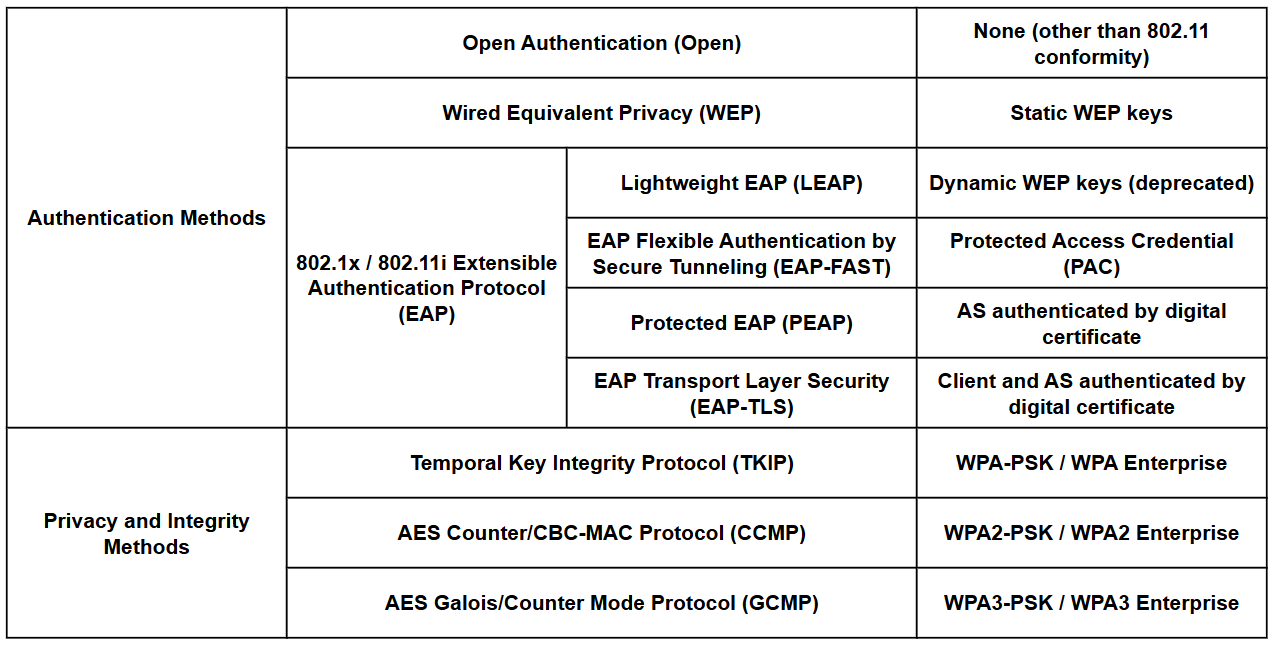
\includegraphics[width=\textwidth,height=7cm]{Wireless_Security}
	\end{figure}


	%Official Standards 																					--subsec:STANDARDS
	\subsection{Official Standards \label{subsec:STANDARDS}}
	\begin{table}[H]
	\centering
	\begin{tabular}{llr}
	\textbf{OFFICIAL STANDARD}		& \textbf{ALTERNATIVE}		& \textbf{REFERENCE}\\\hline
	IEEE 802.3 Copper				& ANSI/TIA-598 Fiber		& \Cref{subsec:CABLING}\\
	IEEE 802.3af/at/bt PoE			& Cisco ILP				& \Cref{tab:POE}\\\hline
	Ethernet II / IEEE 802.3			&					& \Cref{subsec:802.3 ETHERNET}\\
	IEEE 802.2 LLC/SNAP			&					& \Cref{tab:802.2 LLC,tab:802.2 SNAP}\\
	IEEE 802.1Q VLAN Tagging		& Cisco ISL / DTP / VTP		& \Cref{subsec:VLAN TAGGING,subsec:CISCO VTP}\\
	IEEE 802.1AB LLDP			& Cisco CDP			& \Cref{subsec:CDP/802.1AB}\\
	IEEE 802.1D/w STP/RSTP			& Cisco PVST+/PVRST		& \Cref{subsec:802.1D/w}\\
	IEEE 802.1s MSTP				&					&\\
	IEEE 802.3AD LACP			& Cisco PAgP			&\\
	IEEE 802.11 WLANs			& Wi-Fi Alliance			& \Cref{subsec:802.11 WLANS}\\
	IEEE 802.11i EAP				&					& \Cref{fig:WIRELESS SECURITY}\\
	IEEE 802.1x Access Control		&					& \Cref{fig:WIRELESS SECURITY}\\
	ITU HDLC / cHDLC			& \RFC{1661} PPP			& \Cref{subsec:ITU HDLC,subsec:IETF PPP}\\\hline
	RFC \rfc{791}/\rfc{1918} IPv4		& \RFC{2460} IPv6		& \Cref{subsec:IPV4,subsec:IPV6}\\
	\RFC{792} ICMP				& \RFC{4443} ICMPv6		& \Cref{subsec:ICMP}\\
	\RFC{826} ARP				& \RFC{4861} NDP		& \Cref{subsec:ARP,subsec:NDP}\\
	\RFC{2328} OSPFv2			& EIGRP / RIP / BGP / ...		& \Cref{subsec:OSPF}\\
	\RFC{5798} VRRP				& Cisco HSRP / GLBP		&\\
	RFC \rfc{1631}/\rfc{3022} NAT		&					&\\
	\RFC{2475} QoS				&					& \Cref{sec:QOS}\\
	\RFC{3031} MPLS				&					& \Cref{sec:MPLS}\\\hline
	\RFC{768} UDP				& \RFC{793} TCP			& \Cref{subsec:UDP,subsec:TCP}\\\hline
	\RFC{959} FTP				& FTPS / TFTP / SFTP / ...	& \Cref{subsec:FTP}\\
	\RFC{2131} DHCP				& \RFC{3046} DHCP Relay	& \Cref{subsec:DHCP}\\
	\RFC{7230} HTTP				& HTTPS				& \Cref{subsec:HTTP}\\
	\RFC{5424} Syslog				&					& \Cref{subsec:SYSLOG}\\
	\RFC{1065} SNMP				&					&\\
	RFC \rfc{1305}/\rfc{5905} NTP		&					&\\
	\RFC{4301} IPSec				& \RFC{5246} TLS			&\\\hline	
	\end{tabular}\end{table}


	%Example Configuration 																					--subsec:CONFIG
	\newpage
	\subsection{Cisco IOS Configuration Examples \label{subsec:CONFIG}}
	\textbf{Layer 2 Interface Configuration:}
	\begin{lstlisting}
configure terminal
	interface F0/1
		mac-address MAC
		bandwidth KBPS
		duplex {half | full | auto}
		speed {MBPS | auto}
		description TEXT

show interfaces [INT] [status | switchport]
	\end{lstlisting}

	\textbf{VLAN Configuration:}
	\begin{lstlisting}
configure terminal
	vlan VLAN_ID
		name TEXT
		[no] shutdown
	[no] shutdown vlan VLAN_ID
	interface F0/1
		switchport trunk encapsulation {dot1Q | isl | negotiate}
		switchport mode {trunk | dynamic {desirable | auto}}
		switchport nonegotiate
		switchport trunk allowed vlan VLAN_LIST
		switchport trunk native vlan VLAN_ID
		[no] shutdown
	interface range F0/2 - 12
		switchport mode access
		switchport {access | voice} vlan VLAN_ID
		[no] shutdown
	vtp mode {server | client | transparent | off}
	vtp domain TEXT
	vtp password PASSWORD
	[no] vtp pruning
	vtp version 2

show interfaces [INT] [status | switchport | trunk]
show vlan brief
show vlan id VLAN_ID
show vtp {status | password}
	\end{lstlisting}

	\textbf{Link Aggregation Configuration:}
	\begin{lstlisting}
configure terminal
	port-channel load-balance {src-mac | dst-mac | src-dst-mac | src-ip | dst-ip | src-dst-ip | src-port | dst-port | src-dst-port}
	interface range F0/13 - 16
		[no] switchport
		[no] shutdown
		channel-group 1 mode {on | desirable | auto | active | passive}
	interface Po1
		[no] switchport
		[no] shutdown

show etherchannel [CHANNEL] {summary | port-channel}
show etherchannel load-balance
test etherchannel load-balance interface INT mac SRC_MAC DST_MAC
	\end{lstlisting}

	\textbf{Port Security Configuration:}
	\begin{lstlisting}
configure terminal
	errdisable recovery cause psecure-violation
	errdisable recovery interval SECS
	interface range F0/2 - 12
		switchport mode {access | trunk}
		switchport port-security violation {protect | restrict | shutdown}
		switchport port-security maximum MAX
		switchport port-security mac-address {MAC | sticky}
		switchport port-security aging type {absolute | inactivity}
		switchport port-security aging time MINS
		switchport port-security aging static
		switchport port-security
	mac address-table aging-time SECS [vlan VLAN_ID]

show errdisable recovery
show interfaces [INT] [status]
show port-security [interface INT]
show mac address-table aging-time
show mac address-table [static | secure] [vlan VLAN_ID | interface INT]
clear mac address-table dynamic [vlan VLAN_ID | interface INT | address MAC]
	\end{lstlisting}

	\textbf{CDP / LLDP Configuration:}
	\begin{lstlisting}
configure terminal
	[no] {cdp | lldp} run
	{cdp | lldp} timer SECS
	{cdp | lldp} holdtime SECS
	[no] cdp advertise-v2
	interface range F0/2 - 12
		[no] cdp enable
		[no] lldp {transmit | receive}

show {cdp | lldp}
show {cdp | lldp} traffic
show {cdp | lldp} interface [INT]
show {cdp | lldp} neighbors [detail] [INT]
show {cdp | lldp} entry NEIGHBOR
	\end{lstlisting}

	\textbf{Spanning Tree Configuration:}
	\begin{lstlisting}
configure terminal
	errdisable recovery cause bpduguard
	spanning-tree mode {pvst | rapid-pvst | mst}
	spanning-tree pathcost method {long | short}
	spanning-tree [vlan VLAN_ID] root {primary | secondary}
	spanning-tree [vlan VLAN_ID] priority {32768 | 28672 | 24576 | ...}
	spanning-tree portfast [edge | network] [bpduguard | bpdufilter] default
	spanning-tree loopguard default
	interface Po1
		spanning-tree [vlan VLAN_ID] cost PORT_COST
		spanning-tree [vlan VLAN_ID] port-priority PORT_PRIO
		spanning-tree [vlan VLAN_ID] link-type {point-to-point | shared}
		spanning-tree portfast [disable | [edge | network] [default | trunk]]
		spanning-tree {bpduguard | bpdufilter} {enable | disable}
		spanning-tree guard {root | loop | none}

show spanning-tree [bridge | summary]
show spanning-tree [vlan VLAN_LIST | interface INT]
	\end{lstlisting}

	\textbf{Authenticated NTP Configuration:}
	\begin{lstlisting}
configure terminal
	clock timezone CST -6 0
	clock summer-time CDT recurring 2 SUNDAY MAR 02:00 1 SUNDAY NOV 02:00
clock set HH:MM:SS DATE MONTH YEAR
clock {update-calendar | read-calendar}
configure terminal
	ntp authenticate
	ntp authentication-key 1 md5 PASSWORD
	ntp trusted-key 1
	ntp master STRATUM
	ntp {peer | server} {A.B.C.D | HOSTNAME} key 1
	ntp update-calendar
	ntp source loopback 0

show ntp status
show ntp associations [detail]
show {clock | calendar} [detail]
	\end{lstlisting}

	\textbf{Logging and SNMP Configuration:}
	\begin{lstlisting}
terminal monitor
configure terminal
	logging console {0-7 | emergency | alert | critical | error | warning | notification | informational | debug}
	logging monitor {0-7 | emergency | alert | critical | error | warning | notification | informational | debug}
	logging buffered [MEMSIZE] {0-7 | emergency | alert | critical | error | warning | notification | informational | debug}
	logging [host] {A.B.C.D | HOSTNAME}
	logging trap {0-7 | emergency | alert | critical | error | warning | notification | informational | debug}
	[no] service {timestamps | sequence-numbers}
	snmp-server community PASSWORD {ro | rw}
	snmp-server contact TEXT
	snmp-server location TEXT
	snmp-server host {A.B.C.D | HOSTNAME} [trap | inform] version 2c PASSWORD
	snmp-server enable traps TRAPS_LIST

{show | clear} logging
show snmp {community | contact | location | host}
	\end{lstlisting}

	\textbf{DHCP Snooping and DAI Configuration:}
	\begin{lstlisting}
configure terminal
	errdisable recovery cause dhcp-rate-limit
	errdisable recovery cause arp-inspection
	ip dhcp snooping
	ip dhcp snooping vlan VLAN_LIST
	[no] ip dhcp snooping information option
	ip arp inspection vlan VLAN_LIST
	ip arp inspection validate {[src-mac] [dst-mac] [ip]}
	interface Po1
		ip dhcp snooping trust
		ip arp inspection trust
	interface F0/1
		ip arp inspection trust
	interface range F0/2 - 12
		ip dhcp snooping limit rate MAX
		ip arp inspection limit rate MAX [burst-interval SECS]

show ip dhcp snooping [binding]
show ip arp inspection [statistics | interfaces]
	\end{lstlisting}

	\textbf{Layer 3 Interface Configuration:}
	\begin{lstlisting}
configure terminal
	sdm prefer lanbase-routing
	ip routing
	ipv6 unicast-routing
	interface F0/0.SUBINT
		encapsulation dot1q VLAN_ID [native]
		ip address {A.B.C.D M.M.M.M | dhcp}
		{ipv6 enable | ipv6 address {ADDRESS/PREFIX_LENGTH [link-local | anycast] | PREFIX/64 eui-64 | dhcp | autoconfig}}
		[no] shutdown
	interface vlan VLAN_ID
		ip address {A.B.C.D M.M.M.M | dhcp}
		{ipv6 enable | ipv6 address {ADDRESS/PREFIX_LENGTH [link-local | anycast] | PREFIX/64 eui-64 | dhcp | autoconfig}}
		[no] shutdown
	interface F0/1
		[no] switchport
		ip address {A.B.C.D M.M.M.M | dhcp}
		{ipv6 enable | ipv6 address {ADDRESS/PREFIX_LENGTH [link-local | anycast] | PREFIX/64 eui-64 | dhcp | autoconfig}}
		[no] shutdown
		ip helper-address DHCP_SERVER

show sdm prefer
show {ip | ipv6} interface [brief | INT]
show interfaces [INT] [switchport | trunk]
show protocols [INT]
show dhcp lease
show ip default-gateway
show vlans
	\end{lstlisting}

	\textbf{IP Routing Configuration:}
	\begin{lstlisting}
configure terminal
	router ospf 1
		router-id {A.B.C.D | VALUE}
		auto-cost reference-bandwidth MBPS
		maximum-paths 4
		distance 110
		default-information originate [always]
		[no] passive-interface {INT | default}
		[no] network A.B.C.D W.W.W.W area AREA
		[no] shutdown
	interface S0/0/0
		ip ospf 1 area AREA
		ip ospf network {point-to-point | broadcast}
		ip ospf cost PORT_COST
		ip ospf priority 0-255
		ip ospf hello-interval SECS
		ip ospf dead-interval SECS
		ip ospf authentication message-digest
		ip ospf message-digest-key 1 md5 PASSWORD
		ip ospf authentication-key 1
	router rip
		version 2
		no auto-summary
		[no] network NETWORK_ID
		[no] passive-interface INT
		default-information originate
		maximum-paths VALUE
		distance AD
		[no] shutdown
	router eigrp AS_VALUE
		eigrp router-id A.B.C.D
		no auto-summary
		[no] network A.B.C.D [W.W.W.W]
		[no] passive-interface INT
		default-information originate
		maximum-paths VALUE
		variance VALUE
		distance INTERNAL_AD EXTERNAL_AD
		[no] shutdown
	ip route A.B.C.D M.M.M.M {[EXIT_INT] [NEXT_HOP]} [AD] [permanent]
	ipv6 route PREFIX/LENGTH {[EXIT_INT] [NEXT_HOP]} [AD] [permanent]

show {ip | ipv6} protocols
show ip ospf
show ip ospf interface [INT | brief]
show ip ospf neighbor
show ip ospf database
clear ip ospf [PROCESS_ID] process
show {ip | ipv6} route [connected | local | static | ospf | ...] [ADDR]
show ip arp
show ipv6 neighbors
	\end{lstlisting}

	\textbf{VRF Configuration:}
	\begin{lstlisting}
configure terminal
	ip vrf VRF_NAME
	interface F0/0
		ip vrf forwarding VRF_NAME
		ip address {A.B.C.D M.M.M.M | dhcp}
		[no] shutdown
show ip vrf
show ip route vrf VRF_NAME
ping vrf VRF_NAME [ADDRESS]
	\end{lstlisting}

	\textbf{FHRP Configuration:}
	\begin{lstlisting}
configure terminal
	interface F0/0
		standby version 1-2
		standby GROUP_ID ip A.B.C.D
		standby GROUP_ID priority 1-255
		standby GROUP_ID preempt
		standby GROUP_ID description TEXT
		vrrp GROUP_ID ip A.B.C.D [secondary]
		vrrp GROUP_ID priority 1-254
		vrrp GROUP_ID preempt [delay minimum SECS]
		vrrp GROUP_ID description TEXT

show standby [brief]
show standby neighbors [INT]
show vrrp [brief | GROUP_ID]
show vrrp interface INT [brief]
	\end{lstlisting}

	\textbf{DHCP Services Configuration:}
	\begin{lstlisting}
configure terminal
	service dhcp
	ip dhcp excluded-address FIRST_IP [LAST_IP]
	ip dhcp pool POOL_NAME
		network A.B.C.D {M.M.M.M | /CIDR}
		domain-name TEXT
		default-router A.B.C.D
		dns-server A.B.C.D
		lease {DAYS HRS MINS | infinite}
		option 43 ip WLC_IP
		option 66 ip TFTP_IP

show ip dhcp pool POOL_NAME
show ip dhcp binding
	\end{lstlisting}

	\textbf{ACL Configuration:}
	\begin{lstlisting}
configure terminal
	access-list {1-99 | 1300-1999} {permit | deny} {[host] SRC_IP | SRC_IP SRC_WC | any} [log]
	access-list {100-199 | 2000-2699} {permit | deny} {ip | icmp} {host SRC_IP | SRC_IP SRC_WC | any} {host DST_IP | DST_IP DST_WC | any} [log]
	access-list {100-199 | 2000-2699} {permit | deny} {tcp | udp} {host SRC_IP | SRC_IP SRC_WC | any} [{eq | neq | lt | gt | range} SRC_PORT] {host DST_IP | DST_IP DST_WC | any} [{eq | neq | lt | gt | range} DST_PORT] [log]
	access-list {1-199 | 1300-2699} remark TEXT
	ip access-list standard {ACL_NAME | ACL_ID}
		[no] [SEQ] {permit | deny} {[host] SRC_IP | SRC_IP SRC_WC | any} [log]
		[no] [SEQ] remark TEXT
		no SEQ
	ip access-list extended {ACL_NAME | ACL_ID}
		[no] [SEQ] {permit | deny} {ip | icmp} {host SRC_IP | SRC_IP SRC_WC | any} {host DST_IP | DST_IP DST_WC | any} [log]
		[no] [SEQ] {permit | deny} {tcp | udp} {host SRC_IP | SRC_IP SRC_WC | any} [{eq | neq | lt | gt | range} SRC_PORT] {host DST_IP | DST_IP DST_WC | any} [{eq | neq | lt | gt | range} DST_PORT] [log]
		[no] [SEQ] remark TEXT
		no SEQ
	interface S0/0/0
		ip access-group {ACL_ID | ACL_NAME} {in | out}
	line vty 0 15
		access-class {ACL_ID | ACL_NAME} {in | out}

show access-lists
show ip access-lists
	\end{lstlisting}

	\textbf{NAT Services Configuration:}
	\begin{lstlisting}
configure terminal
	interface F0/0
		ip nat inside
	interface S0/0/0
		ip nat outside
	ip nat inside source static INSIDE_LOCAL INSIDE_GLOBAL
	ip nat pool POOL_NAME FIRST_IP LAST_IP netmask M.M.M.M
	access-list 1 permit A.B.C.D [W.W.W.W]
	ip nat inside source list 1 pool POOL_NAME [overload]
	ip nat inside source list 1 interface S0/0/0 overload

show ip nat translations
show ip nat statistics
	\end{lstlisting}

	\textbf{QoS Configuration:}
	\begin{lstlisting}
configure terminal
	class-map [match-all | match-any] CMAP_NAME
		match protocol PROTOCOL
	policy-map PMAP_NAME
		class CMAP_NAME
			set ip dscp {EF | AFXY | CSX | BINARY}
			priority percent BANDWIDTH
			bandwidth percent BANDWIDTH
	interface F0/0
		service-policy {input | output} PMAP_NAME
		
show run | section policy-map
	\end{lstlisting}

	\textbf{WLC WLAN Configuration:}
	\begin{enumerate}
		\item{Create a new WLC Dynamic Interface:}
		\begin{itemize} \itemsep -5pt
			\item{\texttt{Name}\hfill(31 or fewer ASCII characters)}
			\item{\texttt{VLAN ID}\hfill(Integer value 1-1001, 1007-4094 inclusive)}
		\end{itemize}
		\item{Create a new WLC WLAN:}
		\begin{itemize} \itemsep -5pt
			\item{\texttt{Profile Name}\hfill(32 or fewer ASCII characters)}
			\item{\texttt{SSID}\hfill(32 or fewer ASCII characters)}
			\item{\texttt{WLAN ID}\hfill(Integer value 1-512 inclusive)}
		\end{itemize}
		\item{Configure the new WLAN:}
		\begin{itemize} \itemsep -5pt
			\item{Bind the Dynamic Interface to the WLAN.}
			\item{Enable the WLAN on the WLC.}
			\item{Enable broadcasting of the WLAN SSID by APs.}
		\end{itemize}
		\item{Secure the new WLAN:}
		\begin{itemize} \itemsep -5pt
			\item{Set \texttt{Layer 2 Security} to \textbf{WPA+WPA2}, enabling the \texttt{WPA2} checkbox.}
			\item{Set \texttt{WPA2 Encryption} to \textbf{AES/TKIP/CCMP/GCMP}.}
			\item{Enable the \texttt{PSK} checkbox.}
			\item{Set the \texttt{PSK Format} to \textbf{ASCII} and enter the PSK value.}
		\end{itemize}
	\end{enumerate}

%DOCEND
\end{document}